\section{Livello 2 Frame DHLC}


\subsection{Struttura del frame}
\begin{figure}[h!]
    \centering
    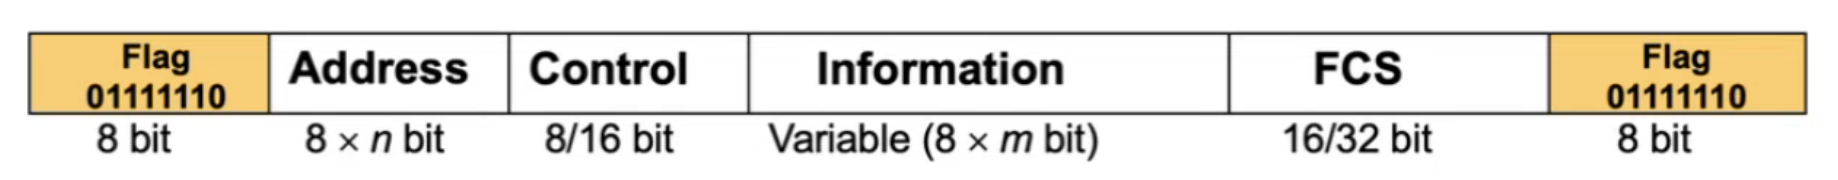
\includegraphics[width=0.8\textwidth]{images/strutturaframe.png}
    \caption{Struttura del frame HDLC}
    \label{fig:struttura-frame}
\end{figure}
\begin{itemize}
    \item flag: sono posti ad inizio e fine frame così da delimitare il frame e far capire a chi lo riceve quando inizia e quando finisce il frame, questi flag sono SEMPRE 8 bit in questa sequenza: 
01111110, ossia 7E in esadecimale
        \item address: indirizzo del trasmettitore, ricevitore o broadcast(se tutti 1)

    \begin{multicols}{2}
        \item control: indica il tipo di frame
        \item information: dati del livello superiore, payload
        \item FCS(frame check sequence): 
    \end{multicols}
\end{itemize}

\subsection{Bit stuffing}
 A proposito dei flag usati nel frame(011111110) che succede se questa sequenza invece fa parte della informazione utile del frame e non come flag delimitatore?

\begin{figure}[h!]
    \centering
    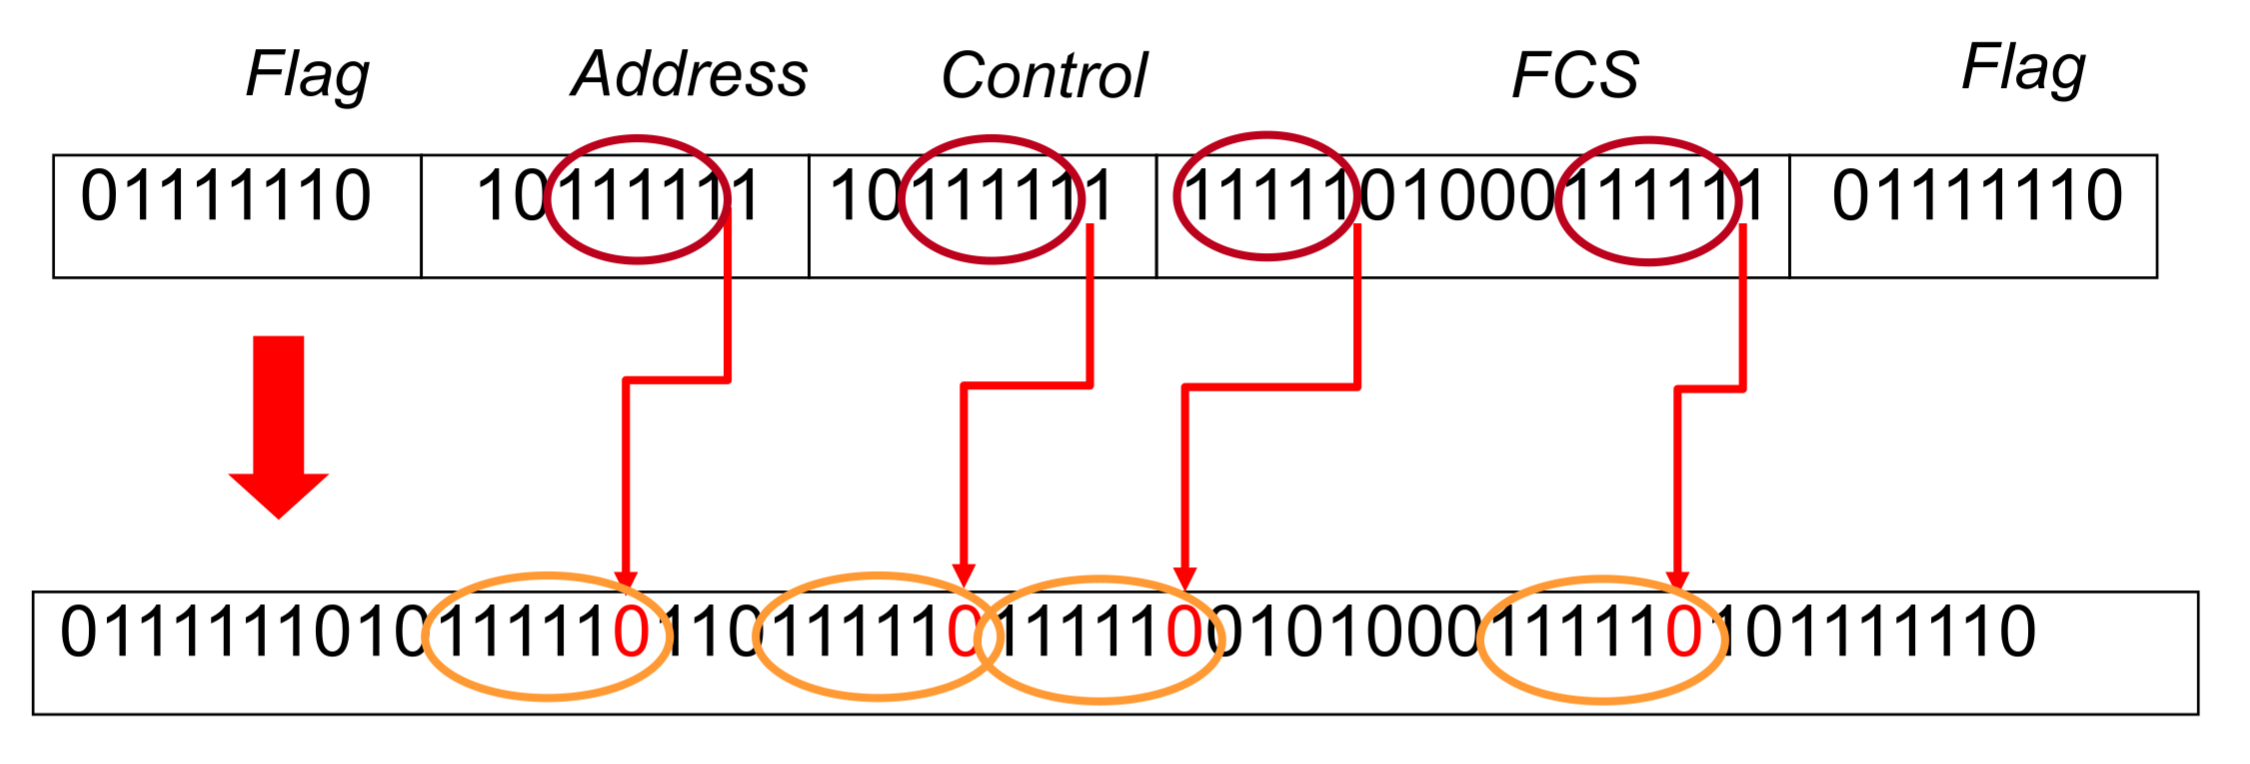
\includegraphics[width=0.8\textwidth]{images/bitstuffing.png}
    \caption{Esempio di bit stuffing}
    \label{fig:bit-stuffing}
\end{figure}
Risolvo inserendo uno 0 ogni cinque 1 ripetuti; questo fa perdere la molteplicità di 8 del frame.

\subsection{Rivelazione dell'errore con CRC}

HDLC numera i frame e usa il protocollo di linea, utilizzando 3 o 7 bit, usando una tecnica di piggybacking per gestire il flusso che viene dalla direzione opposta(finestre di trasmissione e ricezione).

Il CRC è un metodo per il calcolo di somme di controllo (checksum). Il nome deriva dal fatto che i dati d'uscita sono ottenuti elaborando i dati di ingresso i quali vengono fatti scorrere ciclicamente in una rete logica.

Sfrutta l'algebra dei campi finiti ed è utile per l'individuazione di errori casuali nella trasmissione dati (a causa di interferenze, rumore di linea, distorsione), il CRC non è invece affidabile per verificare la completa correttezza dei dati contro tentativi intenzionali di manomissione.
\paragraph{Polinomio generatore}
Un codice CRC è definito dal suo polinomio generatore di ordine r:

esempio r = 3

\begin{equation}
    G(x) = x^3 + x^2 + 1 \quad \Rightarrow \quad 1101
\end{equation}

\subsubsection{Cosa avviene in trasmissione}
 Con una scelta opportuna del polinomio generatore è possibile rilevare errori sul singolo bit etc... ;

 setup del CRC per la trasmissione:

\begin{figure}[htbp]
    \centering
    \begin{minipage}{0.45\textwidth}
        Traduco i bit che compongono header e payload in un polinomio P(x) di coefficienti d; perciò di grado d-1.
    \end{minipage}%
    \hfill
    \begin{minipage}{0.5\textwidth}
        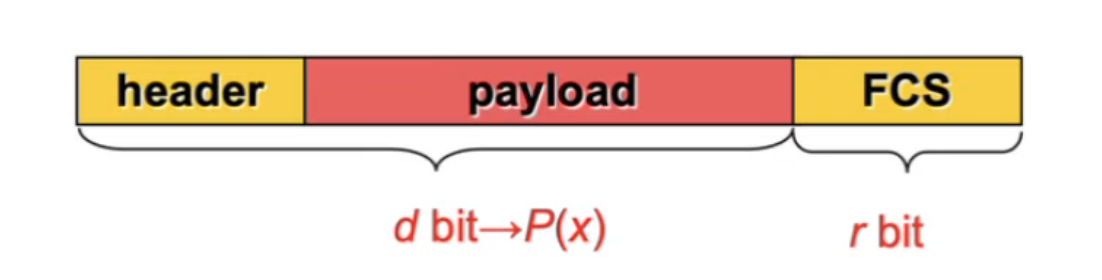
\includegraphics[width=\linewidth]{images/crctrasmissione.png}
        \caption{Schema del calcolo di CRC, P(x)}
    \end{minipage}
\end{figure}

\begin{figure}[htbp]
    \centering
   \begin{minipage}{0.5\textwidth}
        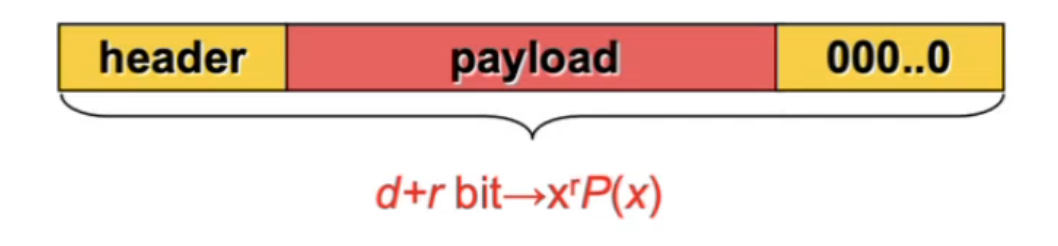
\includegraphics[width=\linewidth]{images/crcricezione.png}
        \caption{Schema del calcolo di CRC, $x^rP(x)$}
    \end{minipage}
    \hfill
     \begin{minipage}{0.45\textwidth}
        Si moltiplica P(x), ricavato qui sopra, per $x^r$(shift di r posizioni, le stesse del poliniomio generatore), ottendo il polinomio $x^rP(x)$ di grado d+r-1, con coefficienti d+r.
      
        In seguito allo shift, il campo FCS del frame sarà costutuito da r zeri.
    \end{minipage}%
\end{figure}

\paragraph{Calcolo e verifica del CRC in trasmissione}
In trasmissione si divide il polinomio $x^rP(x)$ per G(x), il resto di questa operazione[il polinomio R(x)] sono i bit del CRC, da inserire nel FCS del frame.
Vedi operatore XOR appendice basi.

\begin{equation}
    \frac{x^rP(x)}{G(x)} = Q(x) \oplus \frac{R(x)}{G(x)}
\end{equation}


\begin{figure}[htbp]
    \centering
    \begin{minipage}{0.45\textwidth}
        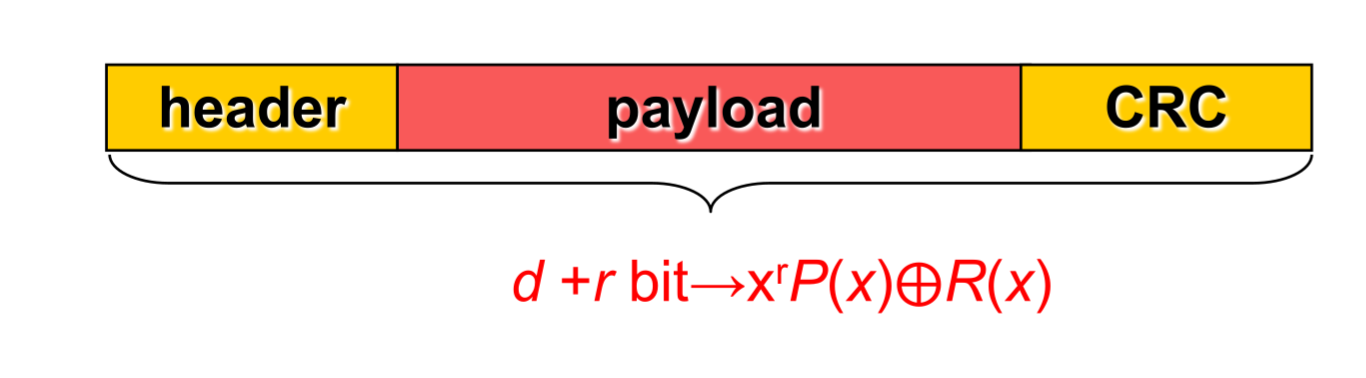
\includegraphics[width=\linewidth]{images/calcolocrc.png}
        \caption{Inserimento bit in FCS}
        \label{fig:calcolo-crc}
    \end{minipage}%
    \hfill
    \begin{minipage}{0.5\textwidth}
        Devo quindi inserire i bit del polonomio R(x) all'interno del FCS, effettuo l'operazione:
\begin{equation}
    P^{Tx} = x^rP(x) \oplus R(x)
\end{equation}
    \end{minipage}
\end{figure}
\newpage
\subsubsection{Verifica CRC}

C'è la necessità di verificare se il CRC calcolato ed inserito nel FCS sia corretto.
\paragraph{Polinomio relativo} è necessario calcolare il polonomio relativo $P^{Rx}(x)$ per verificare CRC; questo polinomio non è altro che la trama di d+r bit ricevuti in ricezione.
\paragraph{Condizione necessaria}
Infine per verificare CRC c'è da tenere a mente la condizione necessaria affinchè il CSC sia corretto, ossia che il resto della divisione tra polinomio relativo[$P^{Rx}(x)$] e polonomio generatore[G(x)] sia nullo:

\begin{equation}
    \frac{P^{Rx}(x)}{G(x)} = Q'(x) \oplus R'(x)
\end{equation}
Può accadere che il resto sia nullo con trama ricevuta errata (la condizione è necessaria, non sufficiente). 

Non si può quindi essere certi della correttezza della trama (c'è sempre una
probabilità non nulla di falso positivo).

Se il resto NON è nullo, invece, c'è la certezza che la trama sia errata
perché la condizione necessaria è stata violata

\paragraph{Dimostrazione condizione necessaria}
Nel caso in cui la trama ricevuta sia corretta, il polinomio che costruiamo da questa trama deve essere uguale al polinomio originale(trama trasmessa), cioè:
\begin{equation}
    P^{Rx}(x) = P^{Tx}(x)
\end{equation}

Se effettuiamo la divisione per il polinomio generatore:

    \begin{equation}
        \frac{P^{Rx}(x)}{G(x)} = \frac{P^{Tx}(x)}{G(x)} = \frac{x^rP(x) \oplus R(x)}{G(x)} = \frac{x^rP(x)}{G(x)} \oplus \frac{R(x)}{G(x)}
    \end{equation}
    \begin{equation}
        \frac{P^{Rx}(x)}{G(x)} = \frac{x^rP(x)}{G(x)} \oplus \frac{R(x)}{G(x)} = Q(x) \oplus \frac{R(x)}{G(x)} \oplus \frac{R(x)}{G(x)} = Q(x)
    \end{equation}

    \subsubsection{Esempio calcolo CRC}
    \begin{figure}[htbp]
        \centering
        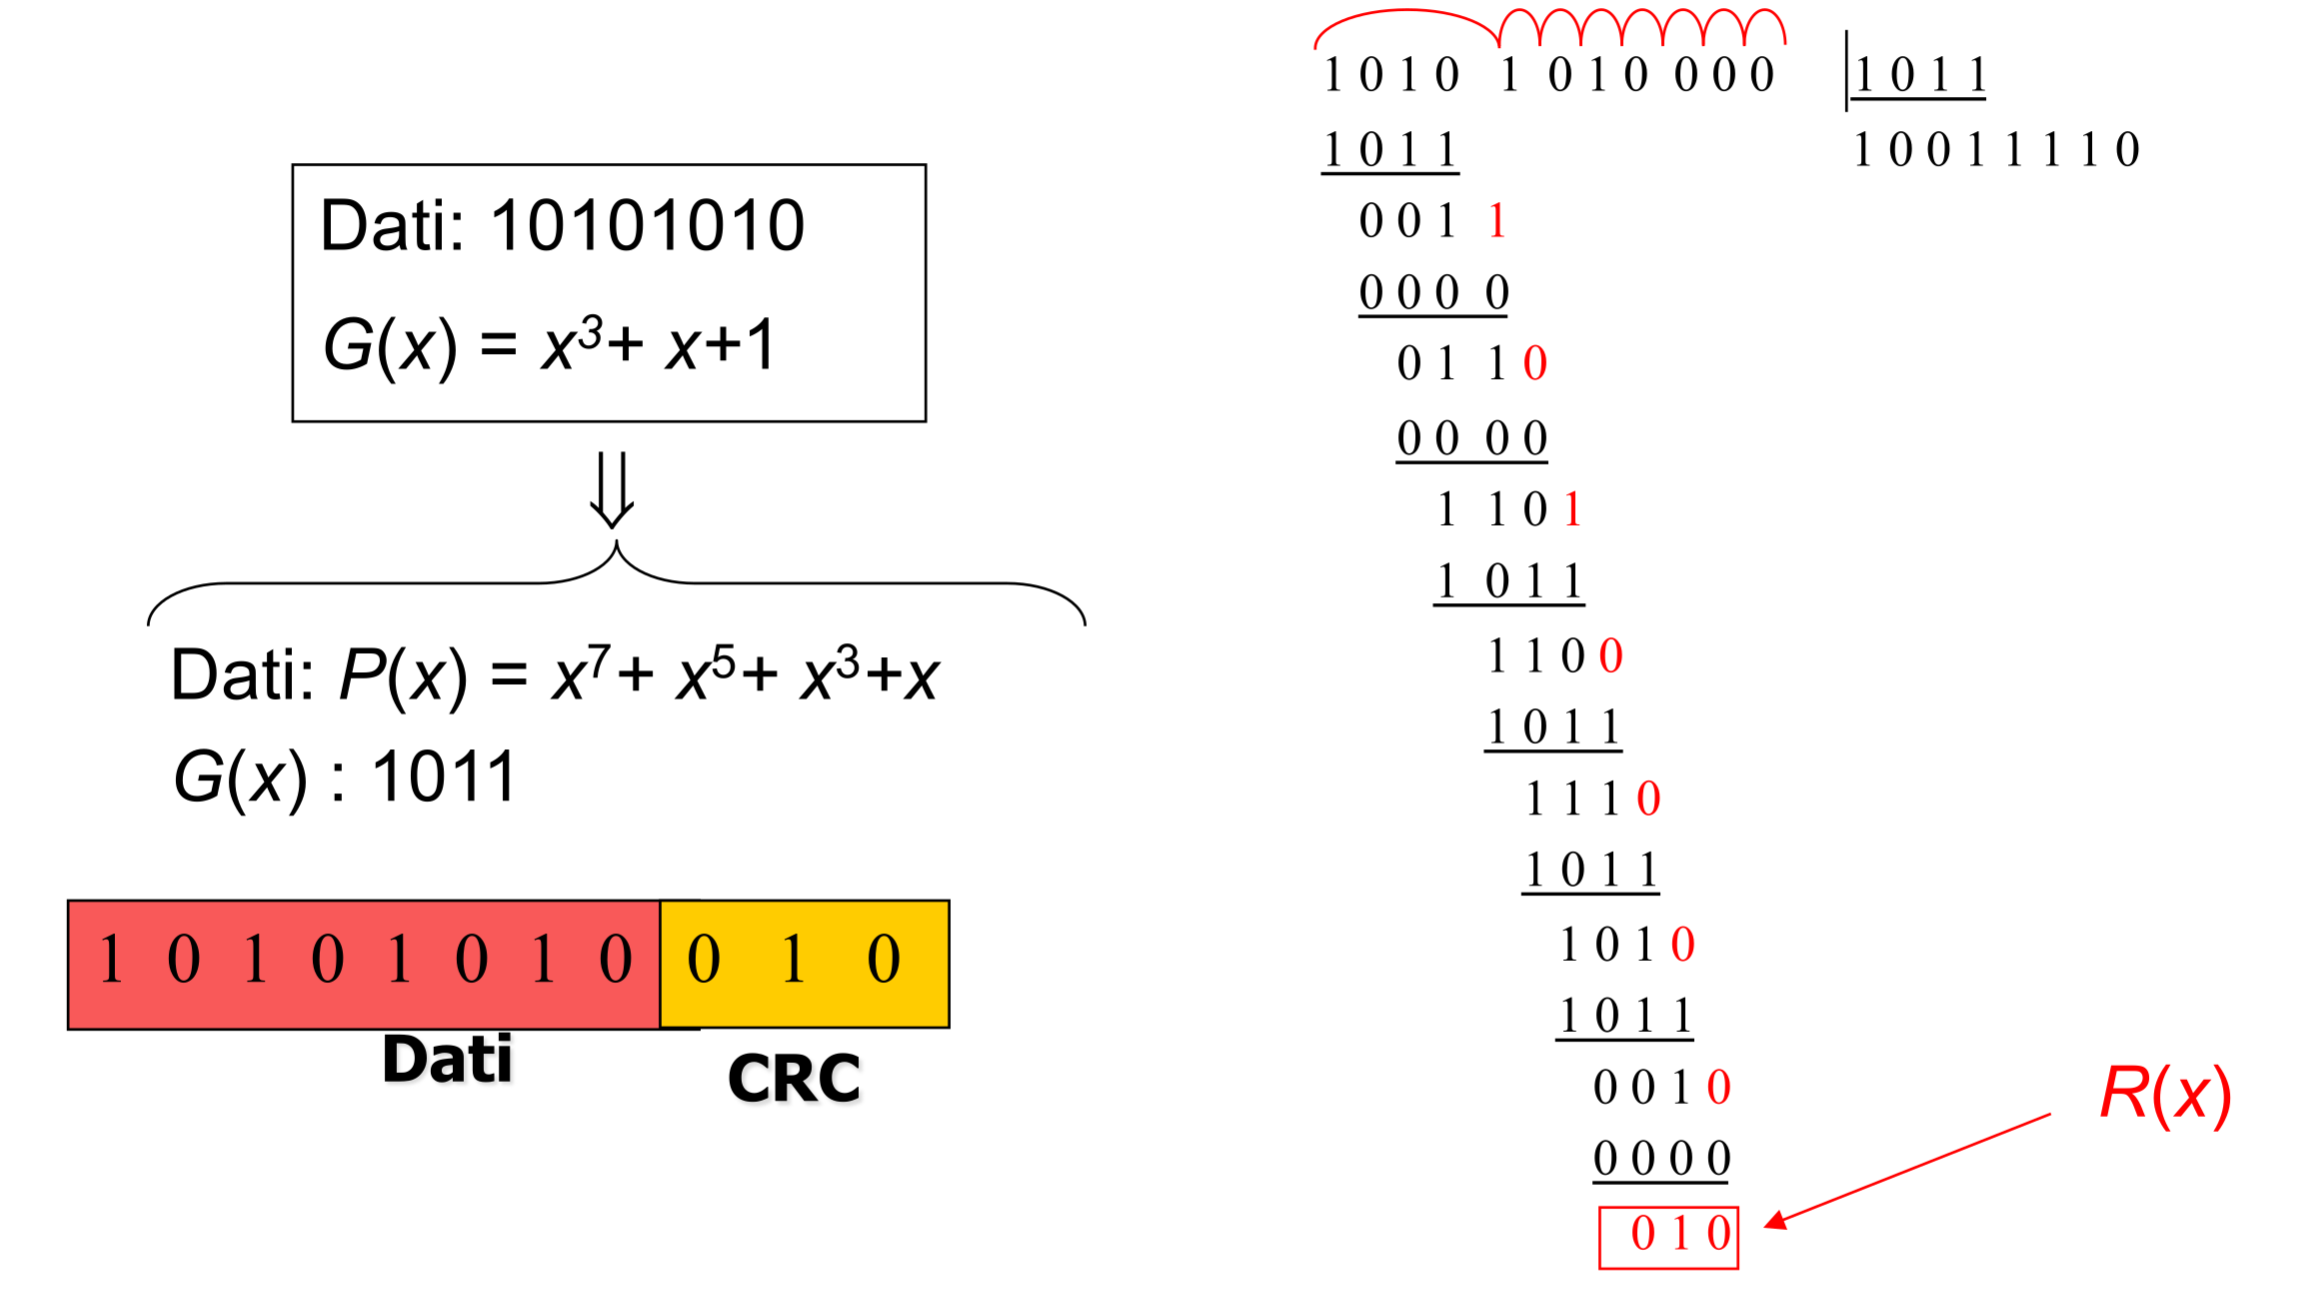
\includegraphics[width=0.8\textwidth]{images/esempiocrc.png}
        \caption{Esempio di calcolo CRC}
        \label{fig:esempio-crc}
    \end{figure}

    \subsection{Protocollo point to point (PPP)}

    \begin{figure}[htbp]
        \centering
        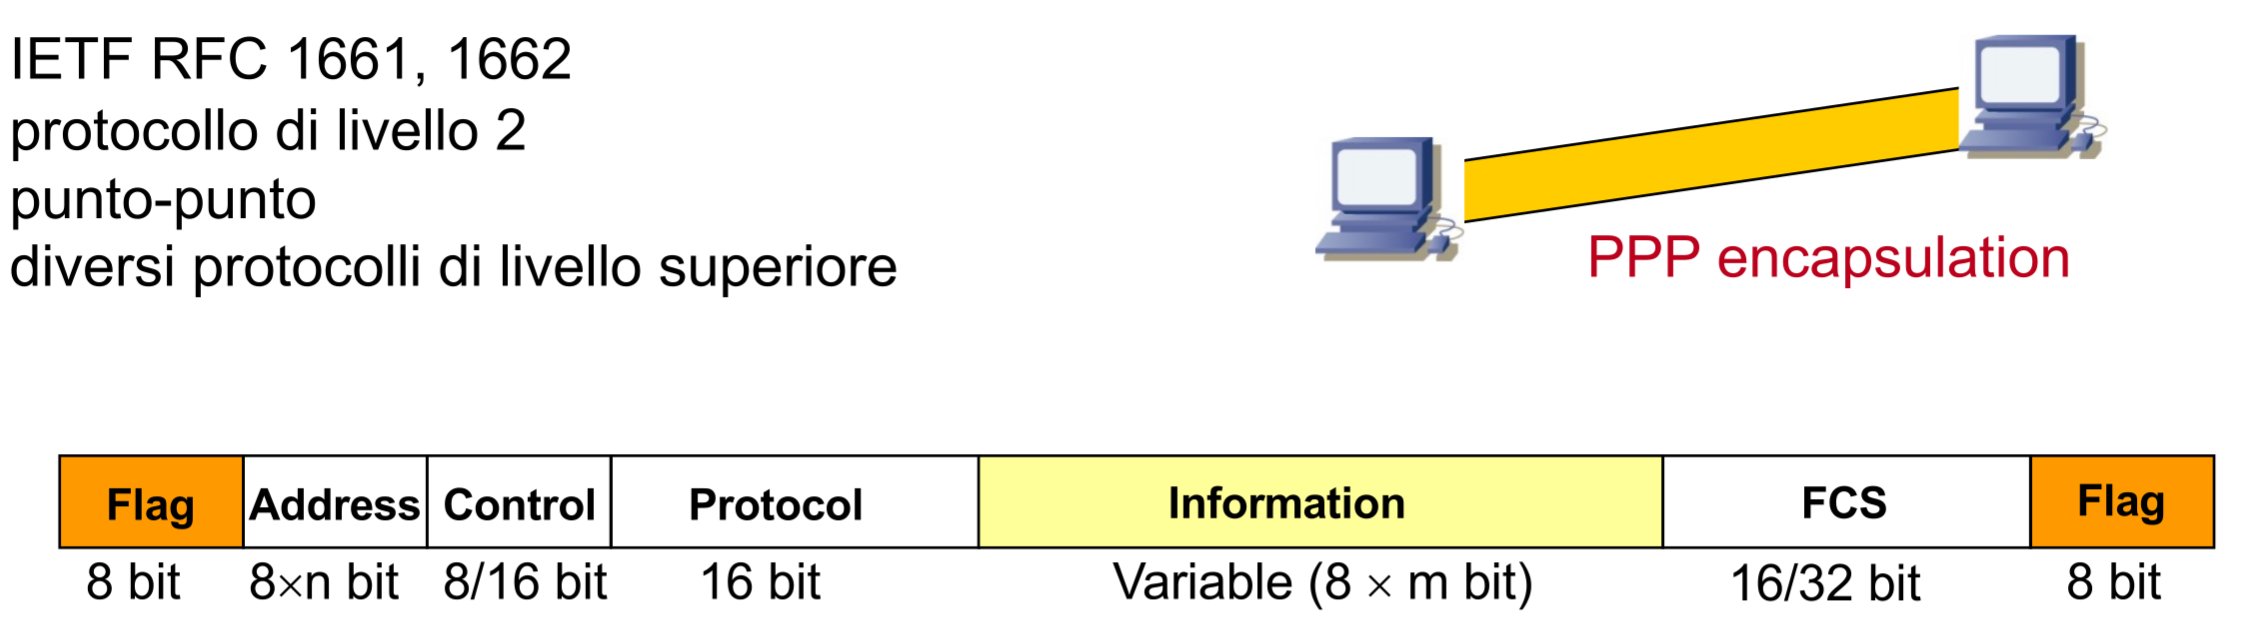
\includegraphics[width=0.85\textwidth]{images/pointtopoint.png}
        \caption{Protocollo Point to Point}
        \label{fig:point-to-point}
    \end{figure}

Il protocollo Point to Point è comunemente usato nello stabilire connessioni dirette tra due nodi.

Il frame è quasi identico a quello del HDLC, ha un campo aggiuntivo, quello protocol: specifica il protocollo di livello 3 che stiamo trasportando.

\paragraph{Network bit order - Big Endian e Little Endian}
A differenza dello standard HDLC, big-endian, il protocollo PPP non è endianness specifico.

L'ordine dei byte (conosciuto anche come big-endian, little-endian o middle-endian a seconda dei metodi differenti), in informatica, indica modalità differenti usate dai calcolatori per immagazzinare all'interno della memoria dati di dimensione superiore al byte;dipende essenzialmente dall'architettura hardware usata.

"I termini big-endian e little-endian derivano dai nomi di due popolazioni che abitavano nelle favolose isole di Lilliput e Blefuscu nel romanzo I viaggi di Gulliver di Jonathan Swift. Queste erano entrate in rivalità per il modo in cui aprivano le uova - rompendo la punta o il fondo: a Lilliput, per editto dell'imperatore il cui figlio una volta si tagliò aprendo un uovo dall'estremità più grande, fu ordinato di aprire le uova dall'estremità più piccola (little endians); a Blefuscu si rifugiarono gli oppositori che volevano conservare la tradizione di rompere le uova dall'estremità più grande (big endians). A causa di questa differenza e della sua legittimazione imperiale era scoppiata tra le due isole una guerra sanguinosa."

\begin{figure}[htbp]
    \centering
    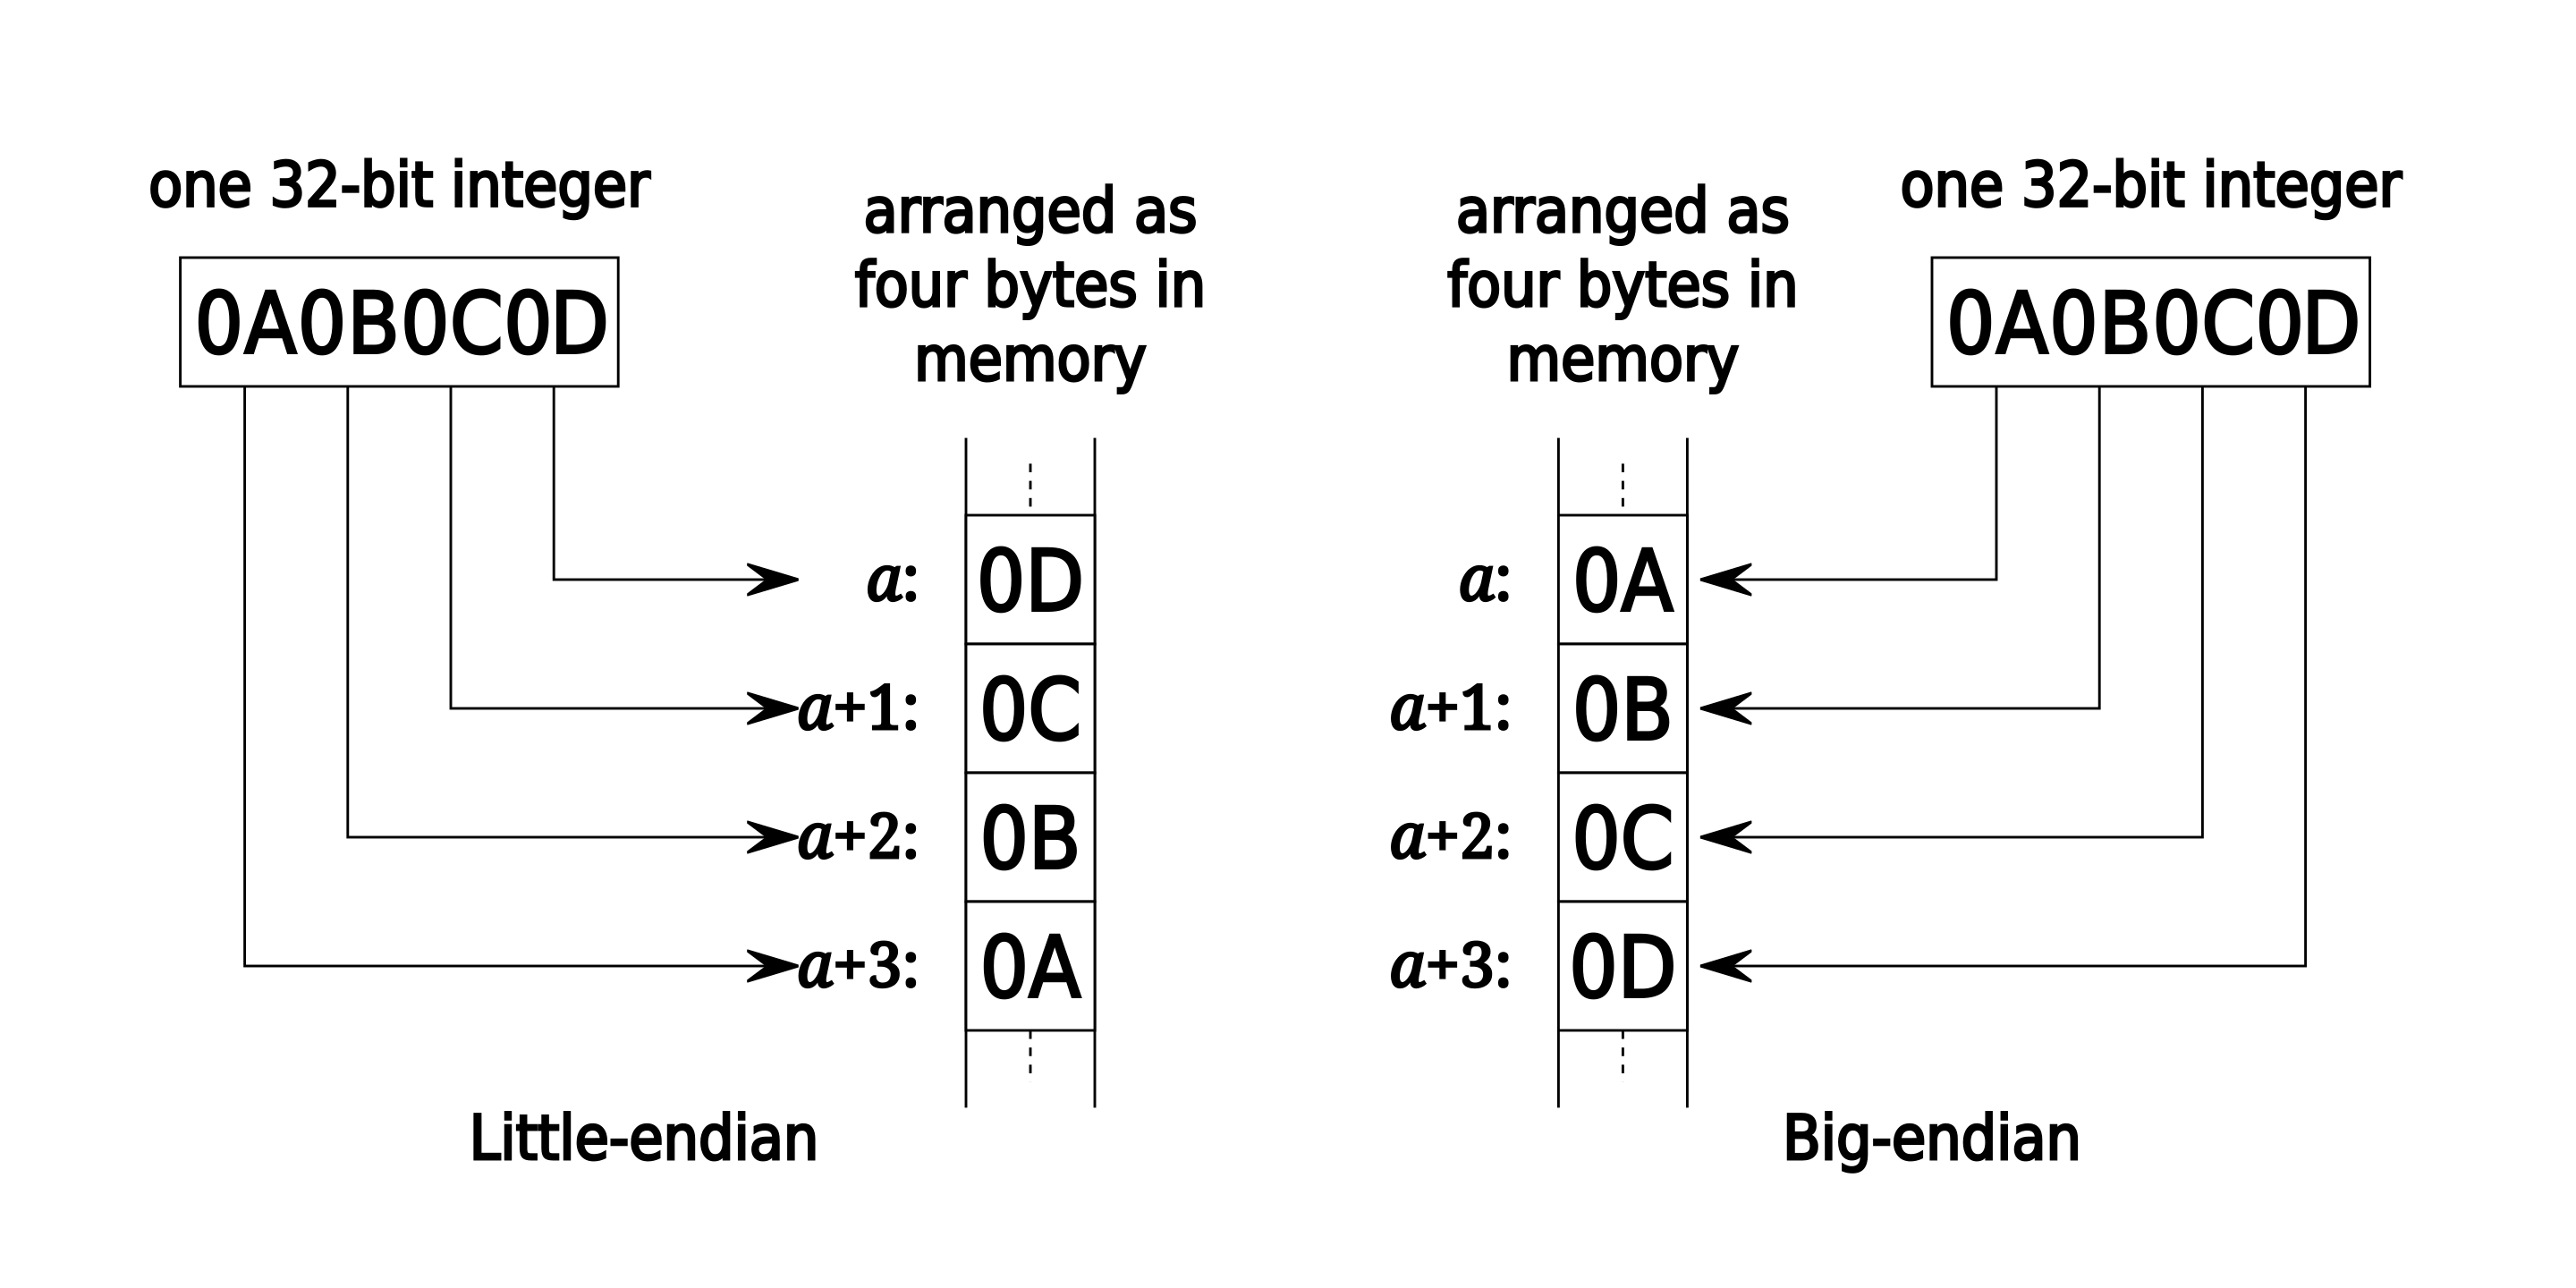
\includegraphics[width=0.8\textwidth]{images/endian.png}
    \caption{Big Endian e Little Endian}
    \label{fig:endian}
\end{figure}
\newpage

    \subsubsection{Byte stuffing}


    Anche qui, vista la struttura del pacchetto molto simile a quella del frame HDLC, c'è il rischio di confondere il dato informativo con un flag; perciò si attua il byte stuffing.

    \paragraph{Sequenza di flag 0x7d}

    Se si vuole evitare la sequenza 0x7e (01111110), si antepone la sequenza di controllo 0x7d (01111101); al posto della sequenza 0x7e inseriamo la sua versione in XOR con la sequenza 0x20 (00100000).
    
    A quel punto avremo individuato la sequenza "pericolosa" all'interno del frame, ossia 0x7e, avremo un identificativo, 0x7d, che ci dice dov'è situata nel frame e la sostituiremo con il suo valore in XOR con 0x20.
     
    Quindi quando all'interno del frame leggo il byte 0x7d, il nuovo flag che indica che c'è stato byte stuffing, non leggiamo 0x7d ma il byte successivo, quello calcolato tramite il 0x7e XOR 0x20.

    In ricezione se applico nuovamente XOR 0x20 al byte precedentemente modificato con lo XOR, allora otterrò nuovamente il byte iniziale, 0x7e.
    
    
    
    \begin{figure}[htbp]
        \centering
        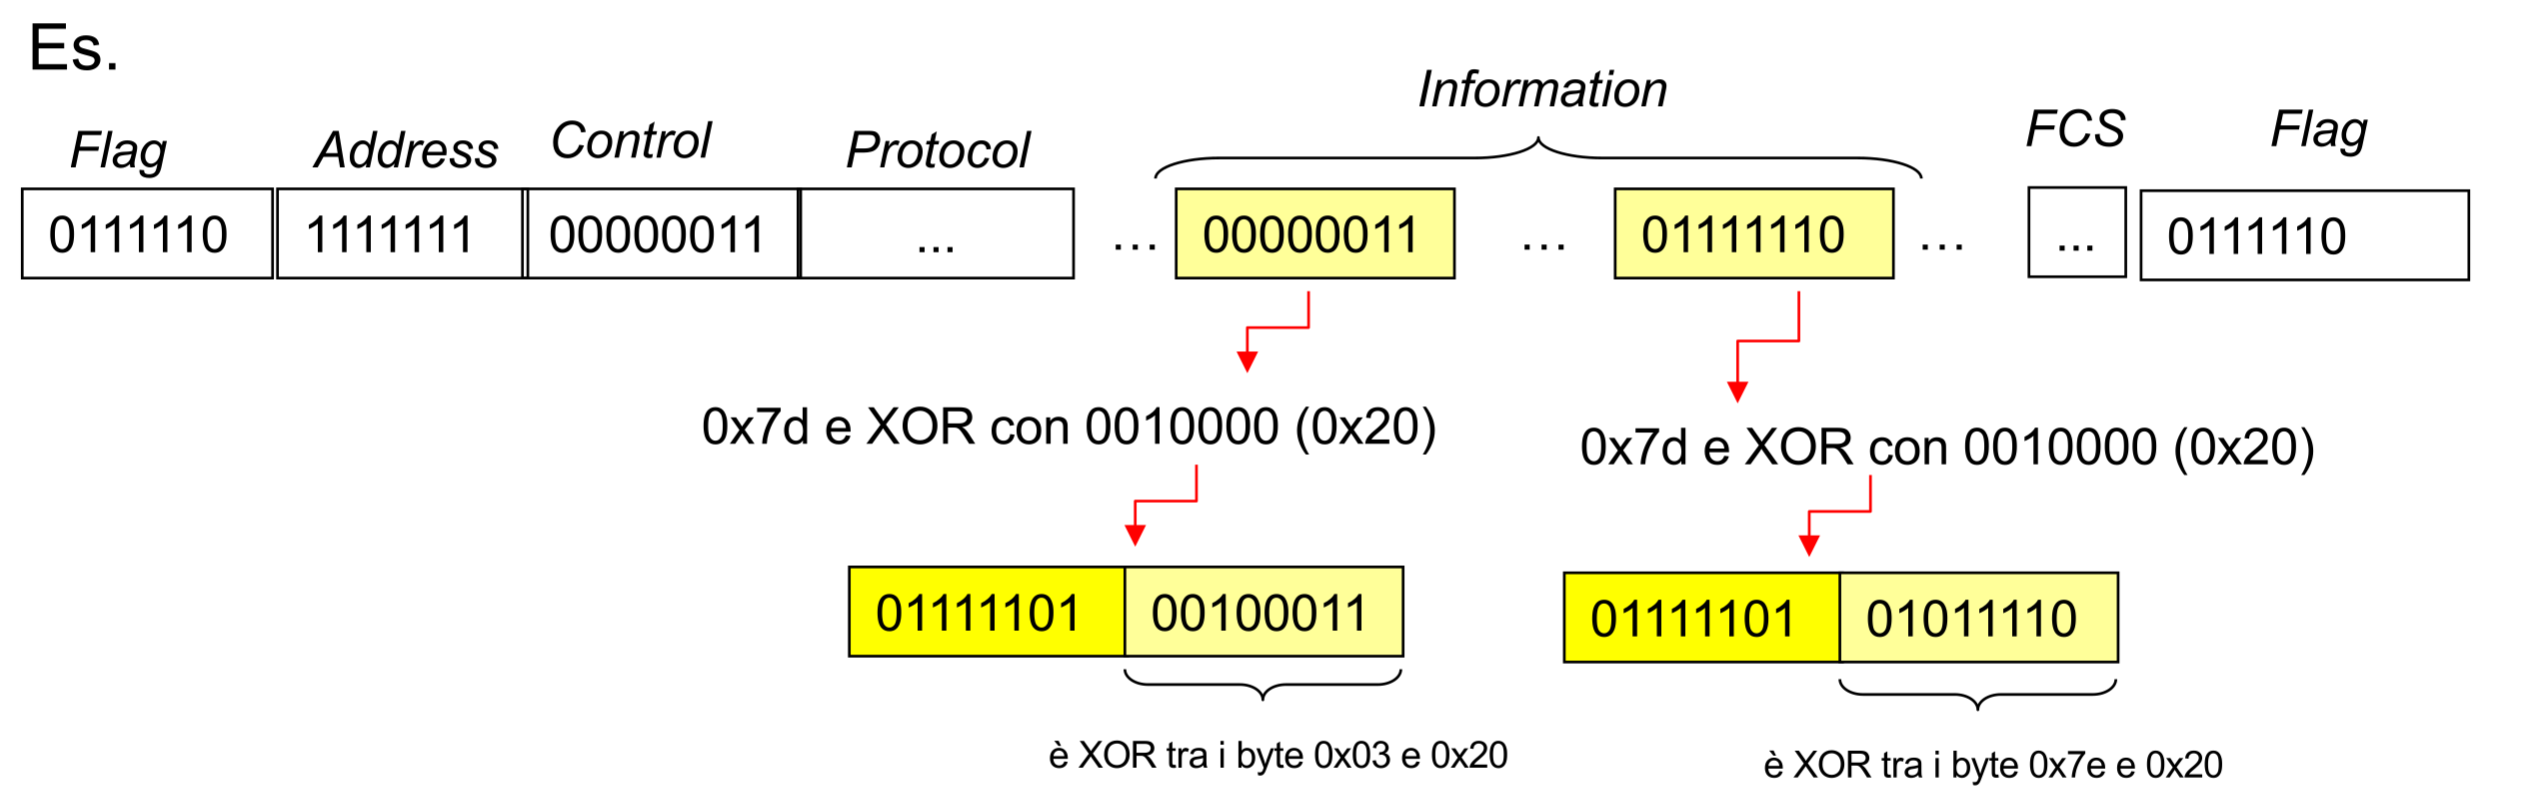
\includegraphics[width=1\textwidth]{images/bytestuffing.png}
        \caption{Esempio di byte stuffing}
        \label{fig:byte-stuffing}
    \end{figure}

    Nel caso in cui incappiamo con una "falsa" sequenza di flag del byte stuffing, ossia 0x7d, la trasmettermo come 0x7d, 0x5d.
     
    \subsubsection{Struttura PPP}

    Il PPP utilizza due protocolli per la gestione del collegamento tra nodi:
    
    \begin{figure}[htbp]
        \centering
        \begin{minipage}{0.45\textwidth}
            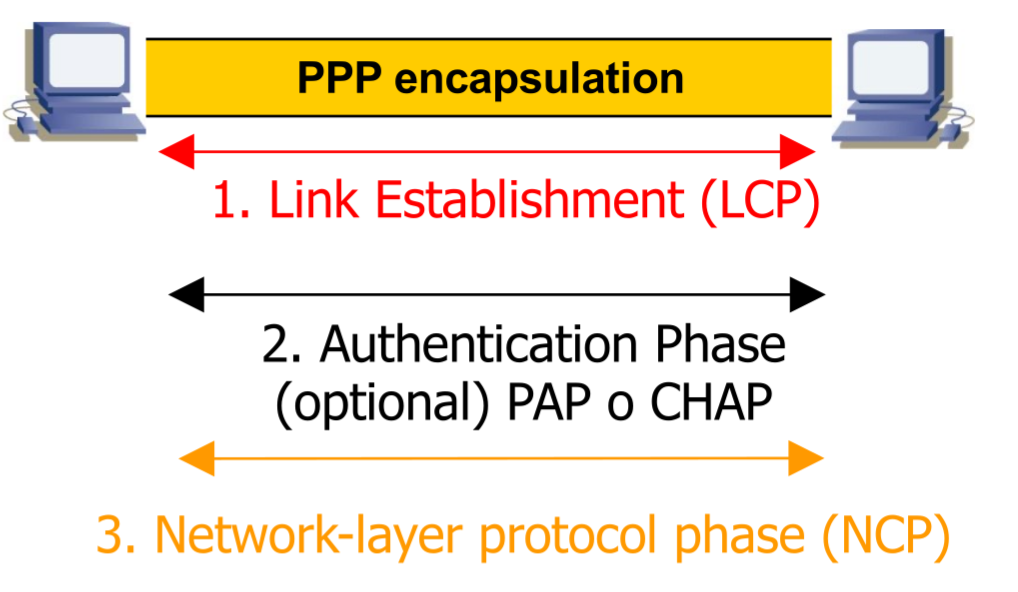
\includegraphics[width=\linewidth]{images/pppencapsulation.png}
            \caption{Encapsulation PPP}
            \label{fig:ppp-encapsulation}
        \end{minipage}%
        \hfill
        \begin{minipage}{0.5\textwidth}
            \begin{itemize}
                \item LCP(Link Control Protocol): grazie al quale si apre la connessione, si ha la verifica della qualità del collegamento e rende possibile l'autenticazione(PAP o CHAP)
                \item NCP(Network Control Protocol): con cui è possible scegliere e configurare uno o più protocolli di rete(es. IP)
            \end{itemize} 

        \end{minipage}
    \end{figure}
\newpage
    \subsubsection{Autenticazioni}
    \begin{figure}[htbp]
        \centering
        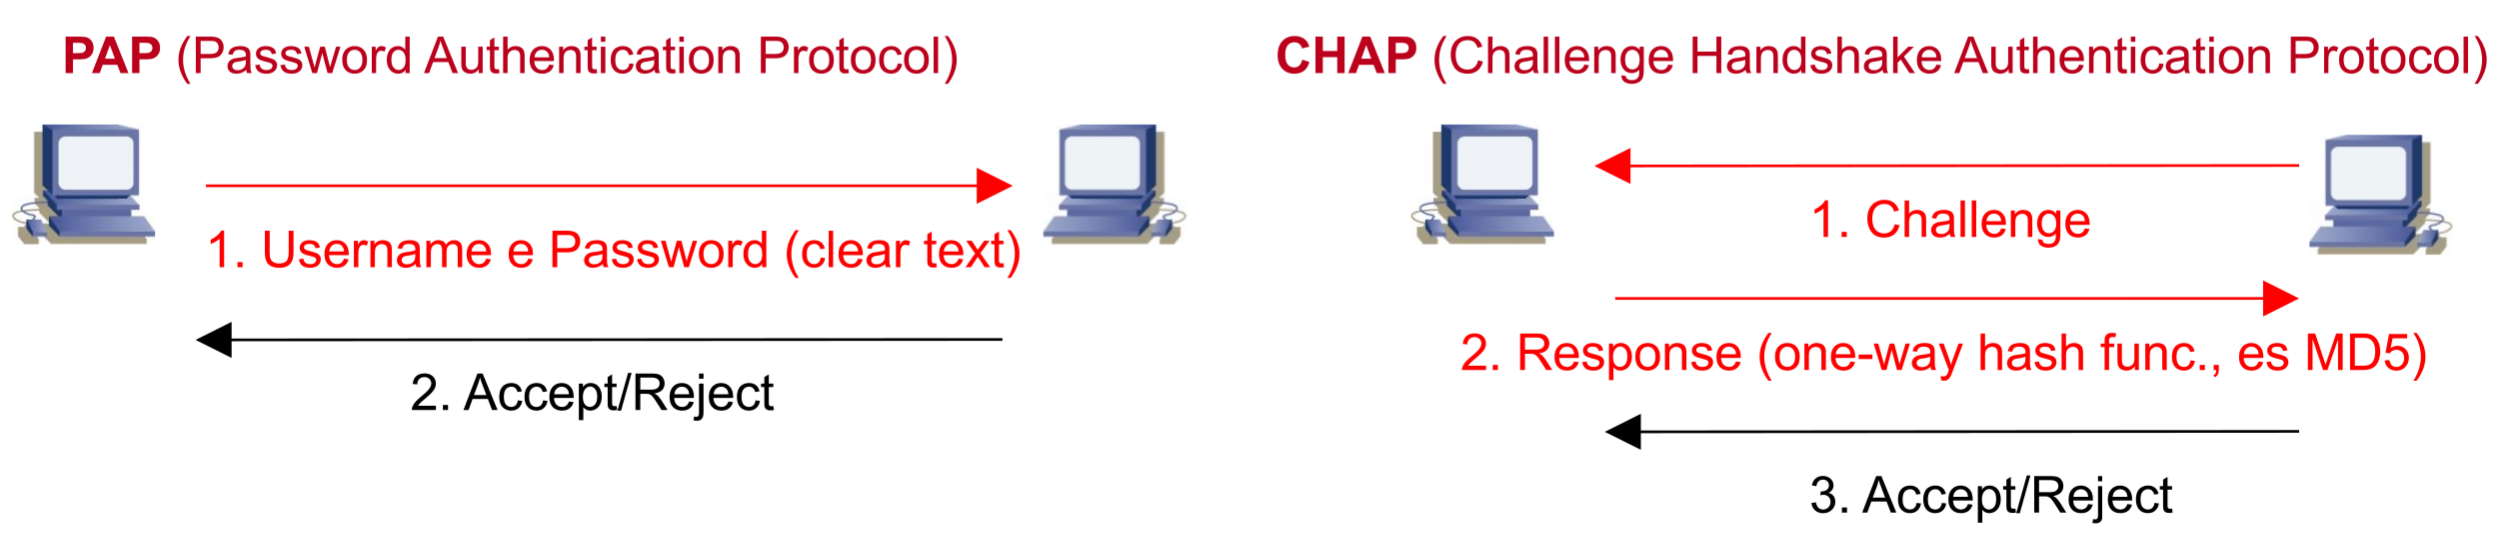
\includegraphics[width=1\textwidth]{images/autenticazionecapchap.png}
        \caption{Autenticazione PAP e CHAP}
        \label{fig:autenticazione-pap-chap}
    \end{figure}
    \paragraph{Autenticazione PAP} 
    Password Authentication Protocol (PAP) invia username e password in chiaro. È semplice ma poco sicuro, poiché le credenziali possono essere intercettate(password e username sono solitamente criptate).

    \paragraph{Autenticazione CHAP} 
    Challenge Handshake Authentication Protocol (CHAP) utilizza un meccanismo di challenge-response con hash per autenticare in modo più sicuro, evitando di trasmettere la password in chiaro.


\section{Protocolli di accesso}
A livello due viene svolto un ruolo importante dai protocolli di accesso, che possono essere di due tipologie:
\begin{itemize}
    \item Accesso ordinato:
    \begin{itemize}
        \item Ogni nodo ha un turno prestabilito per trasmettere, evitando collisioni.
        \item Utilizzato in sistemi come il polling o il token passing.
        \item Garantisce un utilizzo equo del canale, ma può introdurre ritardi se un nodo non ha dati da trasmettere.
    \end{itemize}
    \item Accesso casuale:
    \begin{itemize}
        \item senza rilevazione del canale:
        \begin{itemize}
            \item I nodi trasmettono senza verificare se il canale è libero.
            \item Può portare a collisioni frequenti, come nel protocollo ALOHA puro.
        \end{itemize}
        \item con rilevazione del canale:
        \begin{itemize}
            \item senza rivelazione di collisioni:
            \begin{itemize}
                \item I nodi verificano se il canale è libero prima di trasmettere.
                \item Non rilevano collisioni, quindi i dati persi devono essere ritrasmessi dopo un timeout.
                \item Esempio: Carrier Sense Multiple Access (CSMA).
            \end{itemize}
            \item con rilevazione di collisioni:
            \begin{itemize}
                \item I nodi verificano se il canale è libero e rilevano eventuali collisioni durante la trasm.
                \item In caso di collisione, interrompono la trasm. e ritentano dopo un intervallo casuale.
                \item Esempio: CSMA/CD (utilizzato in Ethernet).
            \end{itemize}
        \end{itemize}
    \end{itemize}
\end{itemize}
\newpage

\subsection{Troughput di rete}
Per valutare le prestazioni di una rete vengono considerati parametri come \dots;
il Troughput, tra questi, è uno dei più rilevanti: è definito come il numero di bit al secondo che giungono corretti; maggiore è questo valore, meglio è per le prestazioni della rete.

Questo valore è alto quando gli errori nei pacchetti che giungono a destinazione sono pochi.

Si parla anche di goodput, ossia il rateo bit al secondo che giungono corretti a destinazione; il Troughput considerava tutti i pacchetti/bit che arrivano a destinazione, anche quelli errati.



\subsubsection{Calcolo del Troughput}

Per il calcolo del Troughput è fondamentale definire alcuni concetti:
\begin{itemize}
    \item frequenza di cifra C: è un paramentro tipico del livello 2 (datalink), rappresenta la capacità del canale su cui sta viaggiando l'informazione, quindi la quantità di bit che possono fisicamente muoversi all'interno del canale
    \item Troughput massimo: è pari alla frequenza di cifra C
    \item $\Lambda_s$: è il numero medio di pacchetti emessi dalla sorgente
    \item $\pi$: la probabilità che il pacchetto arrivi errato o che non arrivi proprio
    \item $\Lambda_T$: Troughput medio
\end{itemize}
\paragraph{Troughput medio packet/s}
Il Troughput medio $\Lambda_T$,misurato in pacchetti al secondo, si calcola come:

\begin{equation}
    \Lambda_T = \Lambda_s (1 - \pi) \quad \text{[packet/s]}
\end{equation}
\paragraph{Troughput medio bit/s}
se desiderassi calcolare il Troughput medio misurato in bit al secondo, ho bisogno di definire il parametro L, ossia la lunghezza media dei pacchetti, allora il Troughput vale:

\begin{equation}
    \Gamma_T = \Lambda_s L (1 - \Pi) \quad \text{[bit/s]}
\end{equation}
\paragraph{Troughput adimensionale}
è anche possibile definire un valore adimensionale del Troughput, che vari da un valore utile che va da 0 ad uno massimo di 1; lo si ottiene normalizzando $\Gamma_s$ alla capacità del canale C; inoltre definiamo:
\begin{itemize}
    \item $T = \frac{L}{C}$ è il tempo medio di trasmissione di un singolo pacchetto
    \item $G = \Gamma_sT$ è il traffico medio normalizzato emesso dalla sorgente
\end{itemize}


\begin{equation}
    S = \frac{\Lambda_s L}{C}(1 - \Pi) = \frac{\Lambda_T}{C} = G(1 - \Pi)
\end{equation}

se S è maggiore di 1 significa che il mittente sta ricevendo più bit di quelli che il canale può supportare.

\newpage

\subsection{Protocollo ALOHA puro}
ALOHA è un protocollo di accesso multiplo casuale senza rilevazione del canale.

Questo protocollo non prevede vincoli all'invio di dati e quindi all'occupazione della banda. Quando una postazione ha dati da trasmettere, li trasmette.

Poiché ogni stazione agisce indipendentemente dalle altre, il successo è determinato unicamente dalla mancata collisione con altre trasmissioni da parte di altre stazioni. Poiché i canali broadcast danno la possibilità di verificare (feedback) se il frame trasmesso è stato ricevuto correttamente oppure se si sono verificate collisioni, la stazione trasmittente ascolta il canale e determina il successo o l'insuccesso della trasmissione. Qualora non sia possibile ascoltare il canale le stazioni si mettono in attesa di un riscontro (ack) da parte del ricevente. Se ci sono collisioni (o se l'ack non arriva entro un tempo di attesa stabilito), i frame corrotti vengono distrutti. Ciò indipendentemente dal livello di corruzione dei dati; quando un frame è stato interessato da collisione, viene eliminato. In questo caso la postazione mittente reinvia il frame dopo un'attesa casuale e si rimette in ascolto sul canale (o attende un ack) fino a quando non stabilisce che il frame è stato ricevuto correttamente.
\subsubsection{Collisioni nel canale condiviso}
\begin{figure}[htbp]
    \centering
    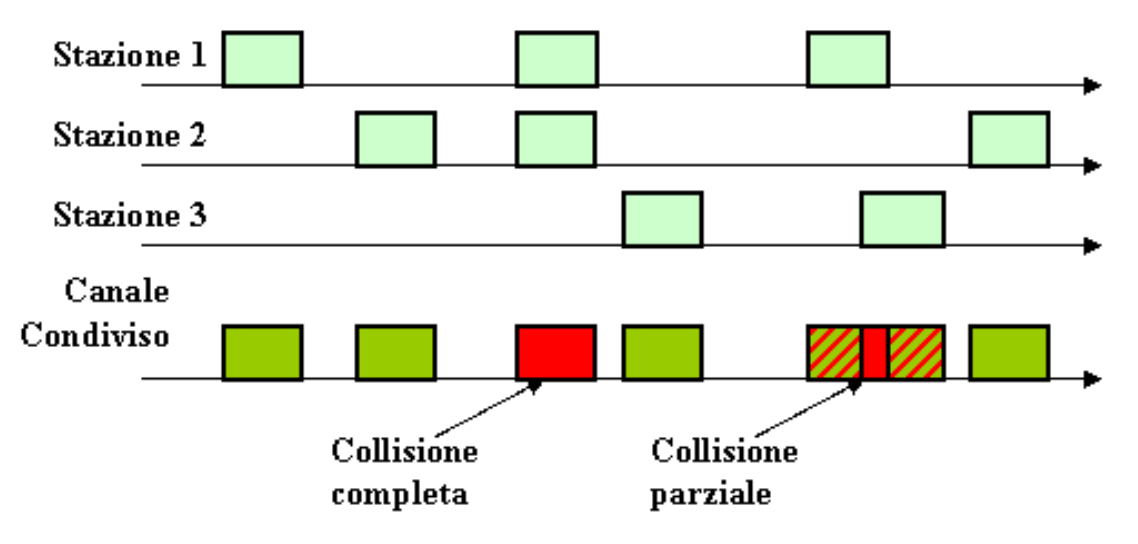
\includegraphics[width=0.8\textwidth]{images/alohacollisioni.png}
    \caption{Collisioni nel protocollo ALOHA}
    \label{fig:aloha-collisioni}
\end{figure}

Le stazioni trasmittenti inviano i loro messaggi lungo il canale condiviso. Se l'intervallo di tempo durante il quale due o più stazioni trasmettono si sovrappone, allora si avrà una collisione; quindi le stazioni coinvolte non riceveranno alcun ack e dovranno perciò ritentare la trasmissione in un istante successivo. 

Per evitare che la collisione si ripeta indefinitamente è opportuno che le stazioni coinvolte tentino la loro ritrasmissione in tempi distinti, in modo da ridurre la probabilità di nuove sovrapposizioni fra i due periodi di trasmissione.

\newpage
\subsubsection{Calcolo del Troughput di ALOHA puro}
Si ipotizza che le stazioni trasmettono sul canale secondo un processo di Poisson, quindi ognuna di esse è un evento indipendente dagli altri; le stazioni trasmettono pacchetti nel canale indipendentemente da ciò che fanno le altre stazioni.

Si suppone anche che ci sia un numero di stazioni molto elevato, che trasmettano tutte nel canale condiviso di interesse; 

ricordando la formula del Troughput medio espresso in pacchetti al secondo: 

\begin{equation}
    \Lambda_T = \Lambda_s (1 - \pi) \quad \text{[packet/s]}
\end{equation}

ci interessa capire quanto può valere $(1 - \pi)$ nel protocollo ALOHA puro, quindi la probabilità che i pacchetti arrivino a destinazione considerando solamente l'effetto della collisione tra pacchetti, non altri fenomeni, poichè si vuole valutare solo l'effetto del protocollo ALOHA sul Troughput.

Per fare ciò considero un nuovo parametro, il periodo di vulnerabilità.

\begin{figure}[htbp]
    \centering
    \begin{minipage}{0.45\textwidth}
        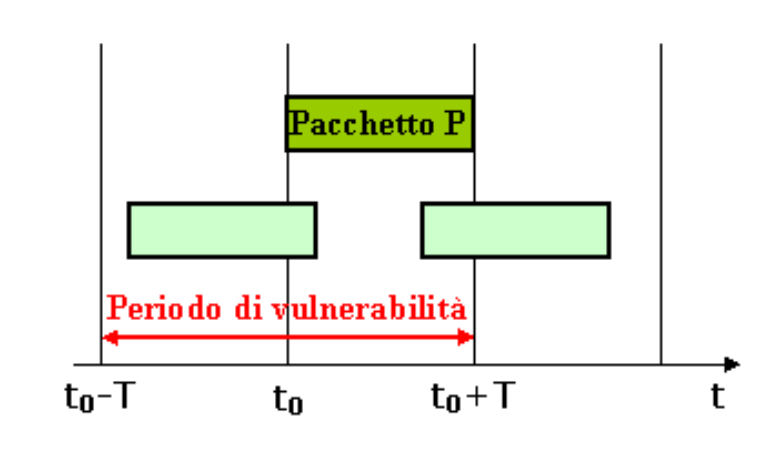
\includegraphics[width=\linewidth]{images/periodovulnerabilita.png}
        \caption{Periodo di vulnerabilità}
        \label{fig:periodo-vulnerabilita}
    \end{minipage}%
    \hfill
    \begin{minipage}{0.5\textwidth}
        Il periodo di vulnerabilità rappresenta l'intervallo di tempo durante il quale una trasmissione(pacchetti verde chiaro) può essere soggetta a collisioni(pacchetto P collide con la trasmissione se rientra nella finestra di 2T). Nel caso del protocollo ALOHA puro, questo periodo è pari a $2T$, dove $T$ è il tempo di trasmissione di un singolo pacchetto. Durante questo intervallo, se un'altra stazione inizia a trasmettere, si verifica una collisione.
    \end{minipage}
\end{figure}

Il valore $(1 - \pi)$ rappresenta quindi la probabilità per la quale nell'intervallo di trasmissione di un pacchetto questo arrivi correttamente(infatti 1 - $\pi$, dove 1 è la probabilità massima per la quale non ci sia collisione, $\pi$ invece rappresenta la probabilità di collisione, più è alta e più andrà a diminuire il valore ideale 1).


Dall'espressione di Poisson($p_0$ rappresenta la probabilità che zero eventi (collisione di pacchetti) si verifichino in un certo intervallo di tempo) si calcola che la probabilità di non avere eventi di collisione nell'intervallo di vulnerabilità 2T è la seguente: 

\begin{equation}
p_k = \frac{(\Lambda t)^k}{k!} e^{-\Lambda t} \Rightarrow p_0 = \frac{(\Lambda_s 2T)^0}{0!} e^{-\Lambda_s 2T} = e^{-2\Lambda_s T} = (1 - \pi)
\end{equation}
\paragraph{Troughput in packet/s}
sostituendolo nella formula di $\Lambda_T$:

\begin{equation}
\Lambda_T = \Lambda_s (1 - \Pi) = \Lambda_s p_0 = \Lambda_s e^{-2 \Lambda_s T} \quad \text{packet/s}
\end{equation}

\paragraph{Troughput in bit/s}

\begin{equation}
    \Gamma_T = \Lambda_s L (1 - \pi) = \Lambda_s L (e^{-2\Lambda_s T}) \quad \text{[bit/s]}
\end{equation}

\paragraph{Troughput adimensionale}

\begin{equation}
    S = \frac{\Lambda_s L}{C}(1 - \Pi) = \frac{\Lambda_T}{C} = G(1 - \Pi) = G(e^{-2\Lambda_s T})
\end{equation}
\newpage

\subsubsection{Prestazioni ALOHA puro}

\paragraph{Andamento funzione $G(e^{-2\Lambda_s T})$} analizzando la funzione 

\begin{figure}[htbp]
    \centering
    \begin{minipage}{0.5\textwidth}
        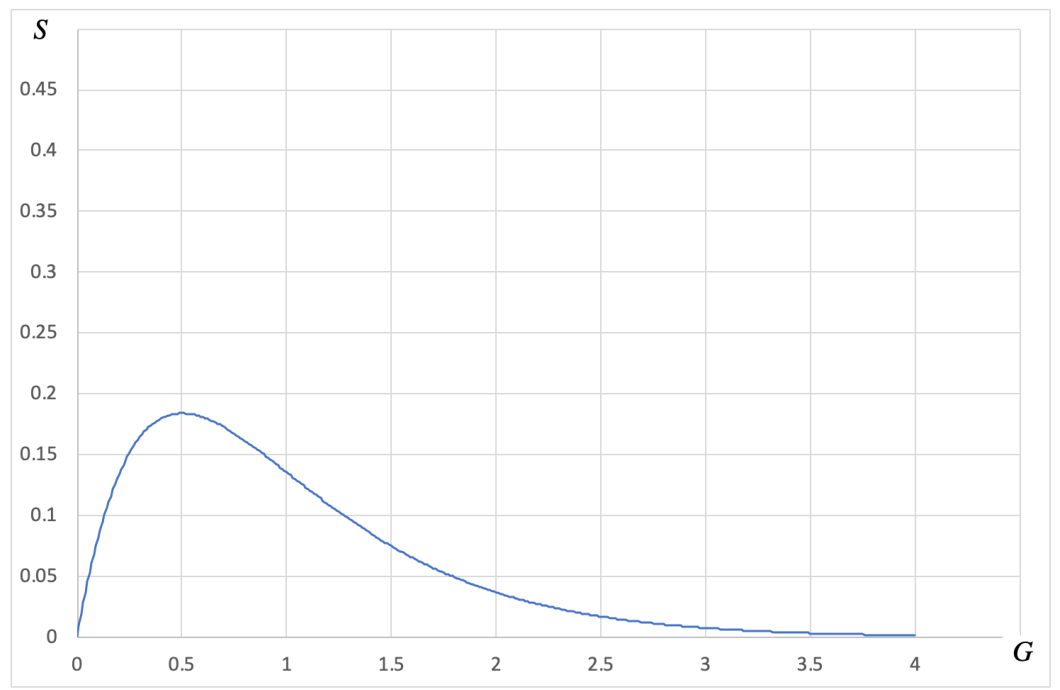
\includegraphics[width=\linewidth]{images/funzionealoha.png}
        \caption{Andamento Troughput normalizzato ALOHA puro}
        \label{fig:funzione-aloha}
    \end{minipage}%
    \hfill
    \begin{minipage}{0.45\textwidth}
        La funzione $S = G e^{-2G}$ ha un massimo per $G = 0.5$, che corrisponde a $S = 0.184$.
        
        Questo significa che il massimo Troughput normalizzato ottenibile con ALOHA puro è circa il 18.4\% della capacità del canale, un valore molto basso dovuto all'elevata probabilità di collisione.
        
        Le prestazioni basse sono dovute al fatto che le stazioni trasmettono senza alcun controllo sul canale.
    \end{minipage}
\end{figure}
\subsubsection{Appendice matematica - distribuzione di Poisson}
La distribuzione di Poisson $\mathcal{P}_\lambda(n)$ è una distribuzione di probabilità discreta data da
\begin{equation}
\mathcal{P}_\lambda(n) = \frac{\lambda^n e^{-\lambda}}{n!} \quad \text{per ogni } n \in {N},
\end{equation}
dove $\lambda$ è il numero medio di eventi per intervallo di tempo, mentre $n$ è il numero di eventi per intervallo di tempo (lo stesso col quale si misura $\lambda$) di cui si vuole la probabilità.

\paragraph{Esempio} Un call center riceve in media 4 chiamate all'ora. Qual è la probabilità che riceva esattamente 2 chiamate in un'ora? ($\lambda = 4$ , $n = 2$)

\begin{equation*}
\mathcal{P}_4(2) = \frac{4^2 \cdot e^{-4}}{2!} = \frac{16 \cdot e^{-4}}{2} \approx \frac{16 \cdot 0.0183}{2} \approx \frac{0.2928}{2} \approx 0.1464
\end{equation*}

\begin{figure}[h!]
    \centering
    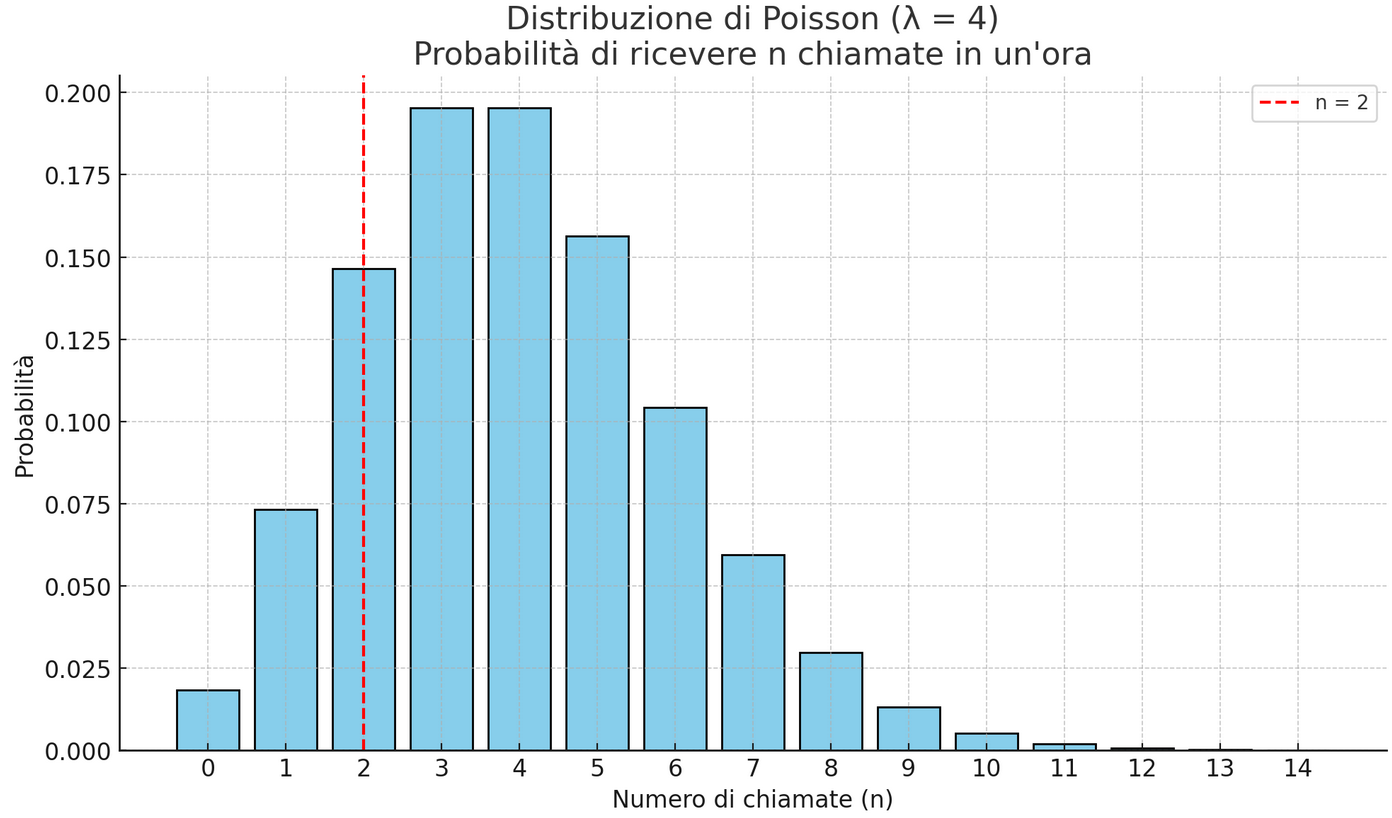
\includegraphics[width=0.8\textwidth]{images/poissongrafico.png}
    \caption{Grafico della distribuzione di Poisson}
    \label{fig:poisson_grafico}
\end{figure}

\newpage

\subsection{Protocollo ALOHA slotted - prestazioni}

Il protocollo Slotted Aloha aggiunge al protocollo Aloha (da cui deriva) un'ulteriore caratteristica, ovvero la suddivisione del tempo in intervalli discreti chiamati slot. 

Ogni stazione è vincolata a cominciare la propria trasmissione all'inizio di uno slot temporale.

Se una stazione ad un certo istante è pronta a trasmettere dovrà attendere necessariamente l'inizio del successivo slot. La conseguenza di tale caratteristica è che due trasmissioni o collidono completamente all'interno dello stesso slot oppure non collidono affatto; il problema delle collisioni parziali non c'è.


\begin{figure}[htbp]
    \centering
    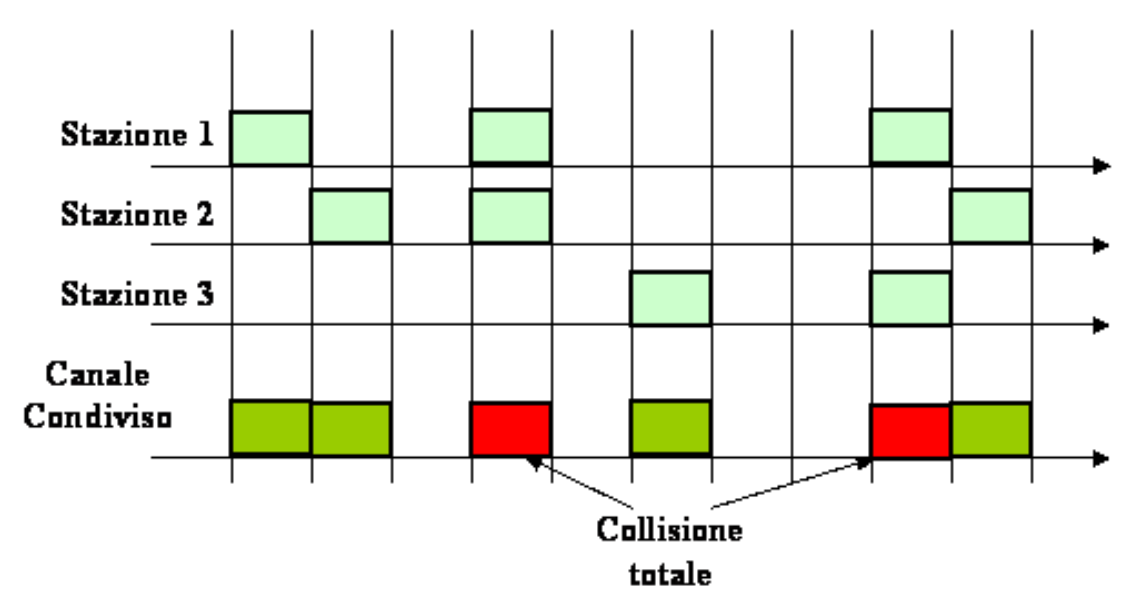
\includegraphics[width=0.77\textwidth]{images/slottedaloha.png}
    \caption{Protocollo ALOHA slotted}
    \label{fig:slotted-aloha}
\end{figure}



\begin{figure}[htbp]
    \centering
    \begin{minipage}{0.43\textwidth}
        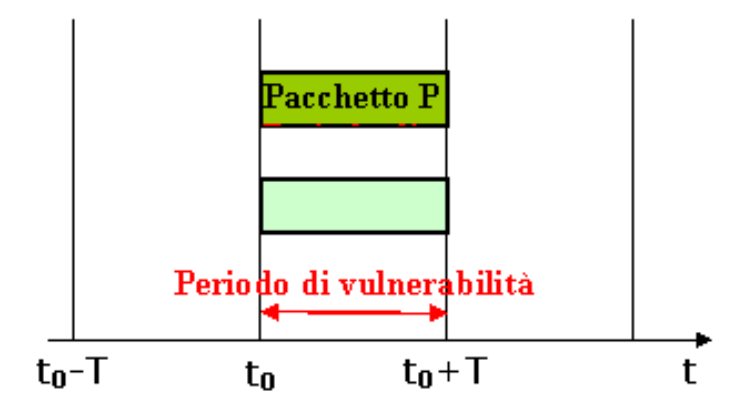
\includegraphics[width=\linewidth]{images/periodoslotted.png}
        \caption{Protocollo ALOHA slotted}
        \label{fig:slotted-aloha}
    \end{minipage}%
    \hfill
    \begin{minipage}{0.45\textwidth}
        \paragraph{Probabilità di collisione}
        Il modello è identico a quello visto per ALOHA, ma stavolta il tempo di vulnerabilità
        si è dimezzato per cui la probabilità di non avere tentativi di trasmissione in T
        \begin{equation}
            p_0 = \frac{(\Lambda_s T)^0}{0!} e^{-\Lambda_s T} = e^{-\Lambda_s T}
        \end{equation}
    \end{minipage}
\end{figure}

\begin{figure}[htbp]
    \centering
    \begin{minipage}{0.425\textwidth}
        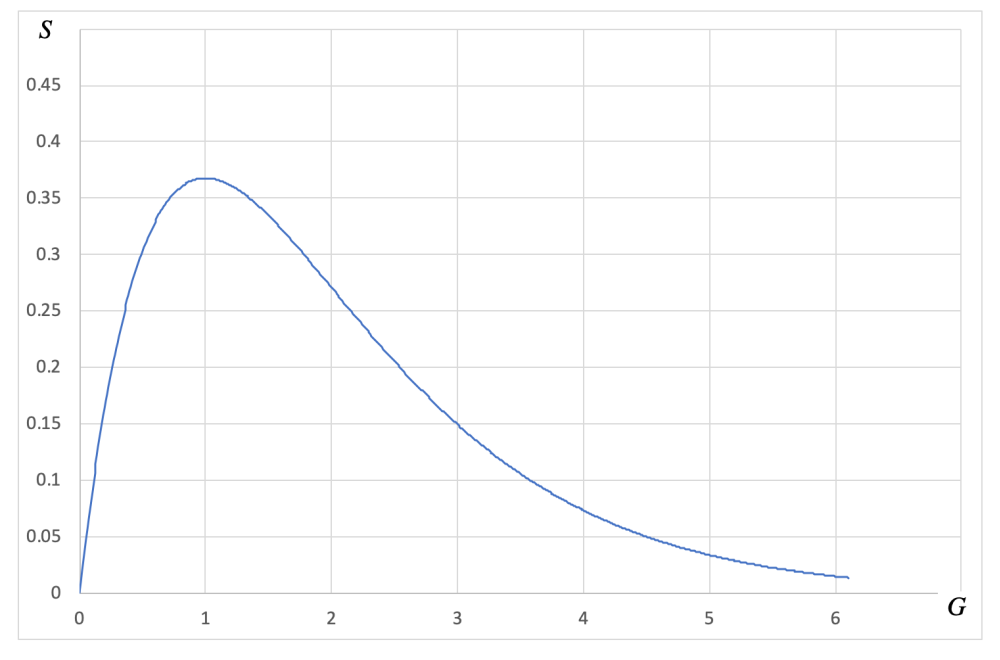
\includegraphics[width=\linewidth]{images/slottedgrafico.png}
        \caption{Protocollo ALOHA slotted}
        \label{fig:slotted-aloha}
    \end{minipage}%
    \hfill
    \begin{minipage}{0.45\textwidth}
        \paragraph{Troughput normalizzato}

\begin{equation}
    S = \Lambda_s \frac{L}{C}p_0 = \Lambda_s \frac{L}{C}e^{-\Lambda_s T} = G e^{-\Lambda_s T}
\end{equation}

Il protocollo Slotted Aloha ha come conseguenza il dimezzamento del periodo di vulnerabilità, che in tal caso è pari a T. L'efficienza massima risulta conseguentemente raddoppiata, pari quindi al 36,8\%.

    \end{minipage}
\end{figure}

\newpage


\subsection{Protocolli Carrier Sense Multiple Access - CSMA (rilevazione canale)}

I protocolli CSMA sono quei protocolli di accesso che rilevano il canale prima di trasmettere, per migliorare l'efficienza ed evitare collisioni con altre trasmissioni.
 
Se rilevando il canale, risulta occupato, allora la stazione può attuare diverse strategie: 
\begin{itemize}
    \item 1-persistent:  continuare a "sentire" il canale finché non lo rileva libero per trasmettere subito dopo
    \item no-persistent: rinviare la trasmissione ad un momento successivo, generalmente scegliendo un intervallo di attesa casuale
    \item p-persistent: scegliere di comportarsi con probabilità p in una delle due modalità precedenti
\end{itemize}
"Può accadere di rilevare il canale come libero, ma nel tempo in cui l'ho rilevato e ho iniziato ad utilizzarlo qualcun'altro potrebbe iniziare a sua volta la comunicazione, c'è quindi da considerare il tempo che impiega l'onda elettromagnetica a viaggiare nel mezzo $v$ e noi a rilevarla $\tau$".

\subsubsection{CSMA/CD - CSMA with collision detection}
Per realizzare il CSMA/CD è necessario che la stazione possa a livello fisico
realizzare una comunicazione full duplex (per essere in grado a livello fisico di
trasmettere e ricevere contemporaneamente, per permettere il listening while talking spiegato successivamente).

La stazione che intende trasmettere verifica che il canale sia libero prima di
trasmettere (sensing del canale del CSMA); 
\paragraph{Listening while talking}
se il canale è libero si trasmette la trama e durante la trasmissione della stessa
(tra l'invio del primo e dell'ultimo bit) si continua ad ascoltare il canale (Listening
while talking)(ascolta se stessa).



\begin{figure}[htbp]
    \centering
    \begin{minipage}{0.5\textwidth}
        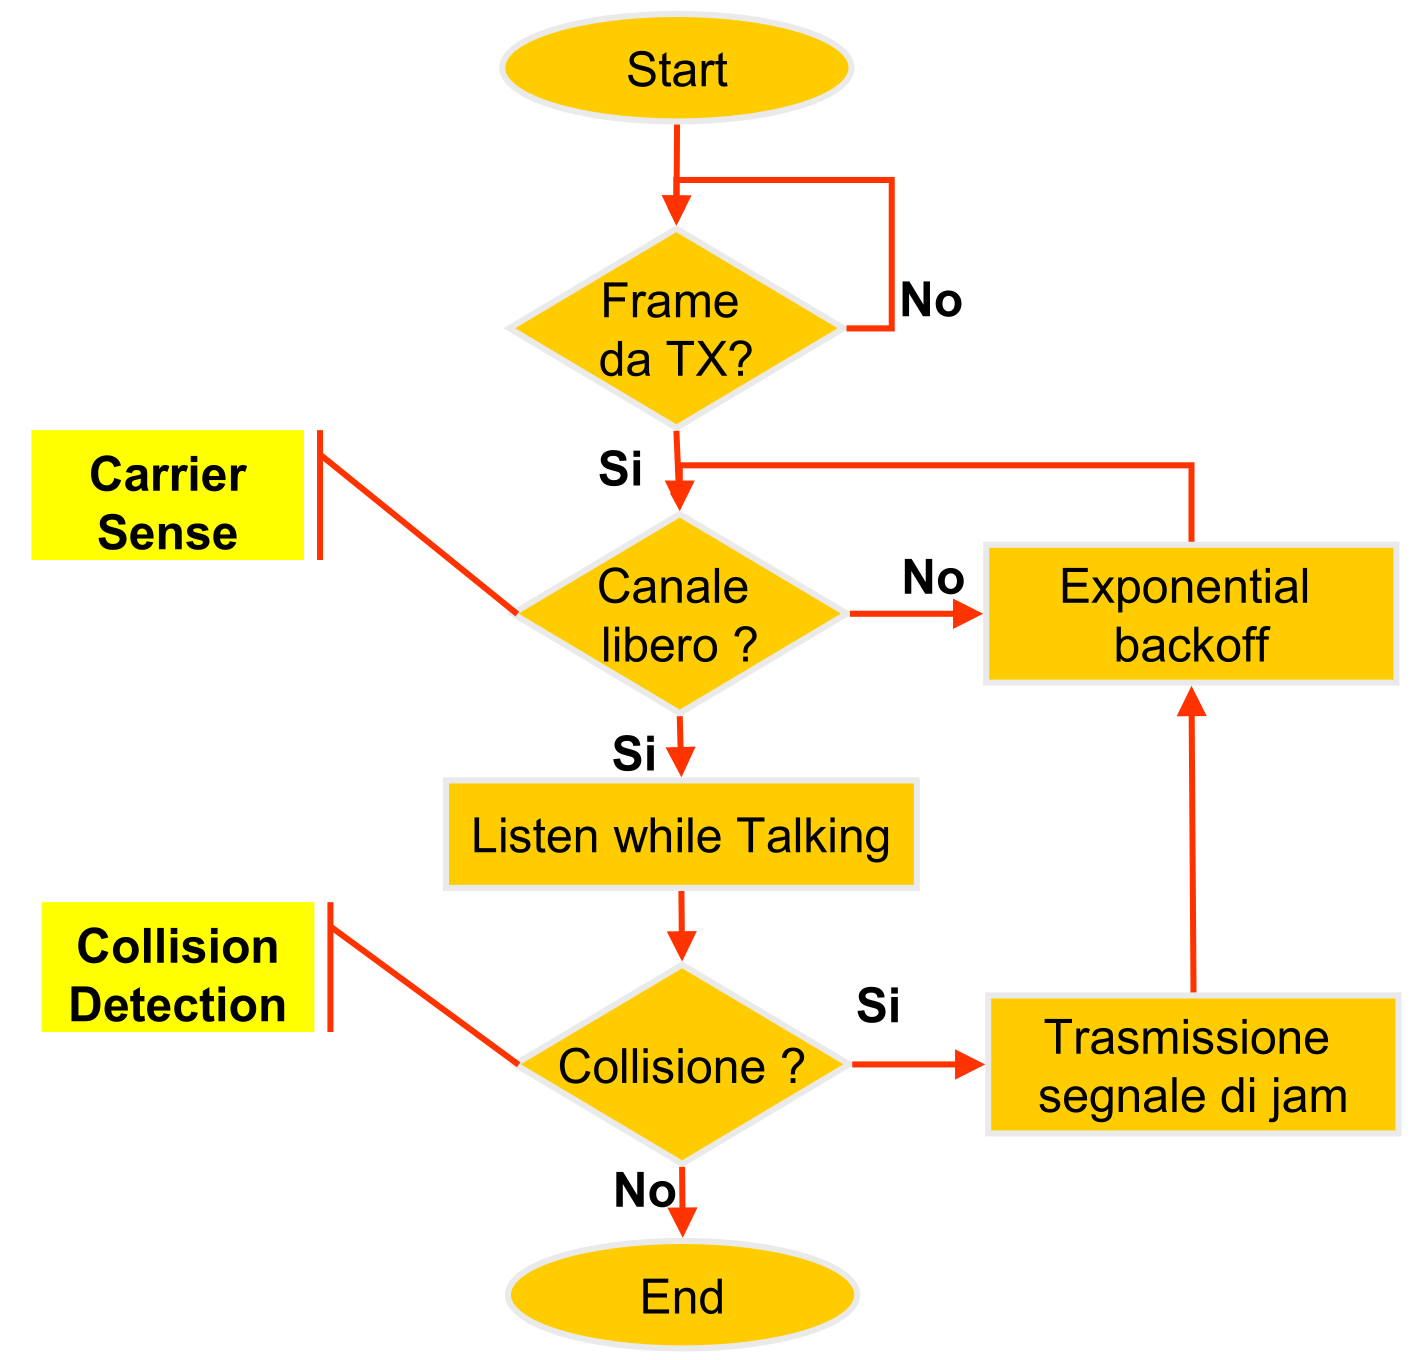
\includegraphics[width=\linewidth]{images/esempiocsmacd.png}
        \caption{Esempio CSMA/CD}
        \label{fig:csma-cd}
    \end{minipage}%
    \hfill
    \begin{minipage}{0.45\textwidth}
        \paragraph{Rilevazione collisione}
Se il segnale "ascoltato" (confronto tra le forme d'onda a livello fisico) è diverso
da quello trasmesso, si rileva la collisione (altra stazione che ha iniziato a
trasmettere sentendo il canale libero). 

In tal caso si può:

\begin{itemize}
    \item interrompere la trasmissione 
    \item inviare un segnale di jam per informare chi sta ascoltando il canale di scartare nel buffer di
ricezione tutti i bit della trama parziale ricevuta
\end{itemize}
    \end{minipage}
\end{figure}
\paragraph{Exponential backoff}
Il tempo di attesa per la rilevazione del canale in seguito ad una collisione viene calcolato in un intervallo $T_{slot}*[0;2^m-1]$ tramite un algoritmo di exponential backoff, per il quale $m = min(n;10)$, m è il numero di ritrasmissioni, n è il numero di collisioni consecutive , $T_{slot}$ è il tempo necessario a trasmettere un frame di lunghezza minima(512 bit). 




\newpage

\subsubsection{Dimostrazione funzionamento collision detection}
Utilizzando il CSMA/CD è necessario che i frame abbiamo una dimensione
superiore ad un valore minimo per garantire il funzionamento del collision
detection.
\begin{figure}[htbp]
    \centering
    \begin{minipage}{0.45\textwidth}
        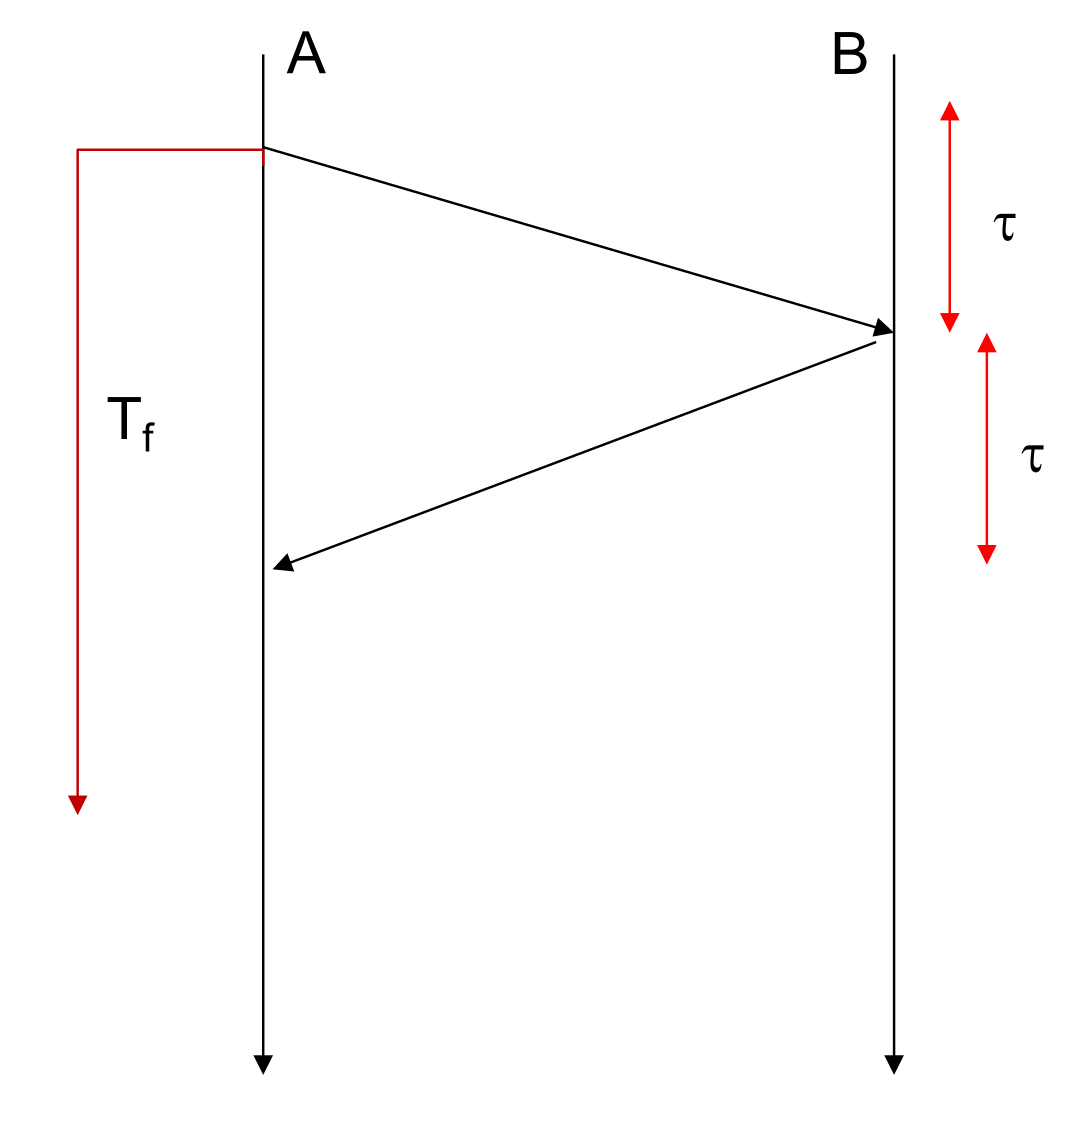
\includegraphics[width=\linewidth]{images/dimostrazionecsma.png}
        \caption{Dimostrazione collision detection}
        \label{fig:dimostrazione-csma}
    \end{minipage}%
    \hfill
    \begin{minipage}{0.5\textwidth}



A e B comunicano nei tampi $\tau$(valore massimo, caso peggiore);
il primo bit inviato da A arriva a B dopo $\tau$ secondi.

Nel caso peggiore B ascolta il canale un istante($\epsilon$) prima che il bit di A arrivi a B, perciò B vedrà che il canale è libero, non sapendo che un'istante dopo arriveranno i bit di A, causando quindi una collisione.

B si accorge della collisione e manda un jam, impiegando $\tau$ per "avvisare" A.

A può apire che il jam che riceve è dovuto ad una collisione con la sua trasmissione solo se la sua trasmissione ($T_f$) dura almeno quanto il tempo che ha impiegato il suo primo bit di trasmissione ed il jam di B, perciò: $T_f  \geq 2\tau$ 

\begin{equation}
 T_f = \frac{L_f}{C} \geq 2\tau = \frac{2d}{v} \implies L_f \geq \frac{2dC}{v}
\end{equation}

        %Si supponga che A inizi a trasmettere al tempo t=0 e che B inizi a trasmettere al tempo $t = t_{prop}$ ($t_{prop}$ è il tempo di propagazione del segnale).

        %A rileverà la collisione al tempo $2t_{prop}$ (tempo necessario al segnale di B per raggiungere A).

        %Per garantire il funzionamento del collision detection, è necessario che A stia ancora trasmettendo quando rileva la collisione.

        %Quindi, la durata minima di un frame deve essere tale che la stazione trasmittente continui ad occupare il canale per almeno $2t_{prop}$.

        %Se la durata della trasmissione è inferiore a $2t_{prop}$, la collisione potrebbe non essere rilevata.
    \end{minipage}
\end{figure}
\subsubsection{CSMA/CA - CSMA with collision avoidance}
\paragraph{Duration}
L'obiettivo del CSMA/CA è diminuire il numero di collisioni.

In questa versione di CSMA, in cui c'è rilevazione del canale prima di trasmettere, se il canale è libero inizia la trasmissione inserendo la durata stimata della trasmissione del singolo frame (considerando anche i tempi di propagazione e la trasmissione del frame di riscontro) in un campo "duration" dell'header del frame.

\paragraph{Network allocation vector(NAV) - virtual sensing} Tutte le altre stazioni che condividono il canale ascoltano il frame e settano un
loro orologio interno, detto NAV, pari al valore del duration letto.

Finchè il NAV non si azzera non iniziano altre trasmissioni poiché si sa che il canale è occupato.
\begin{figure}[htbp]
    \centering
    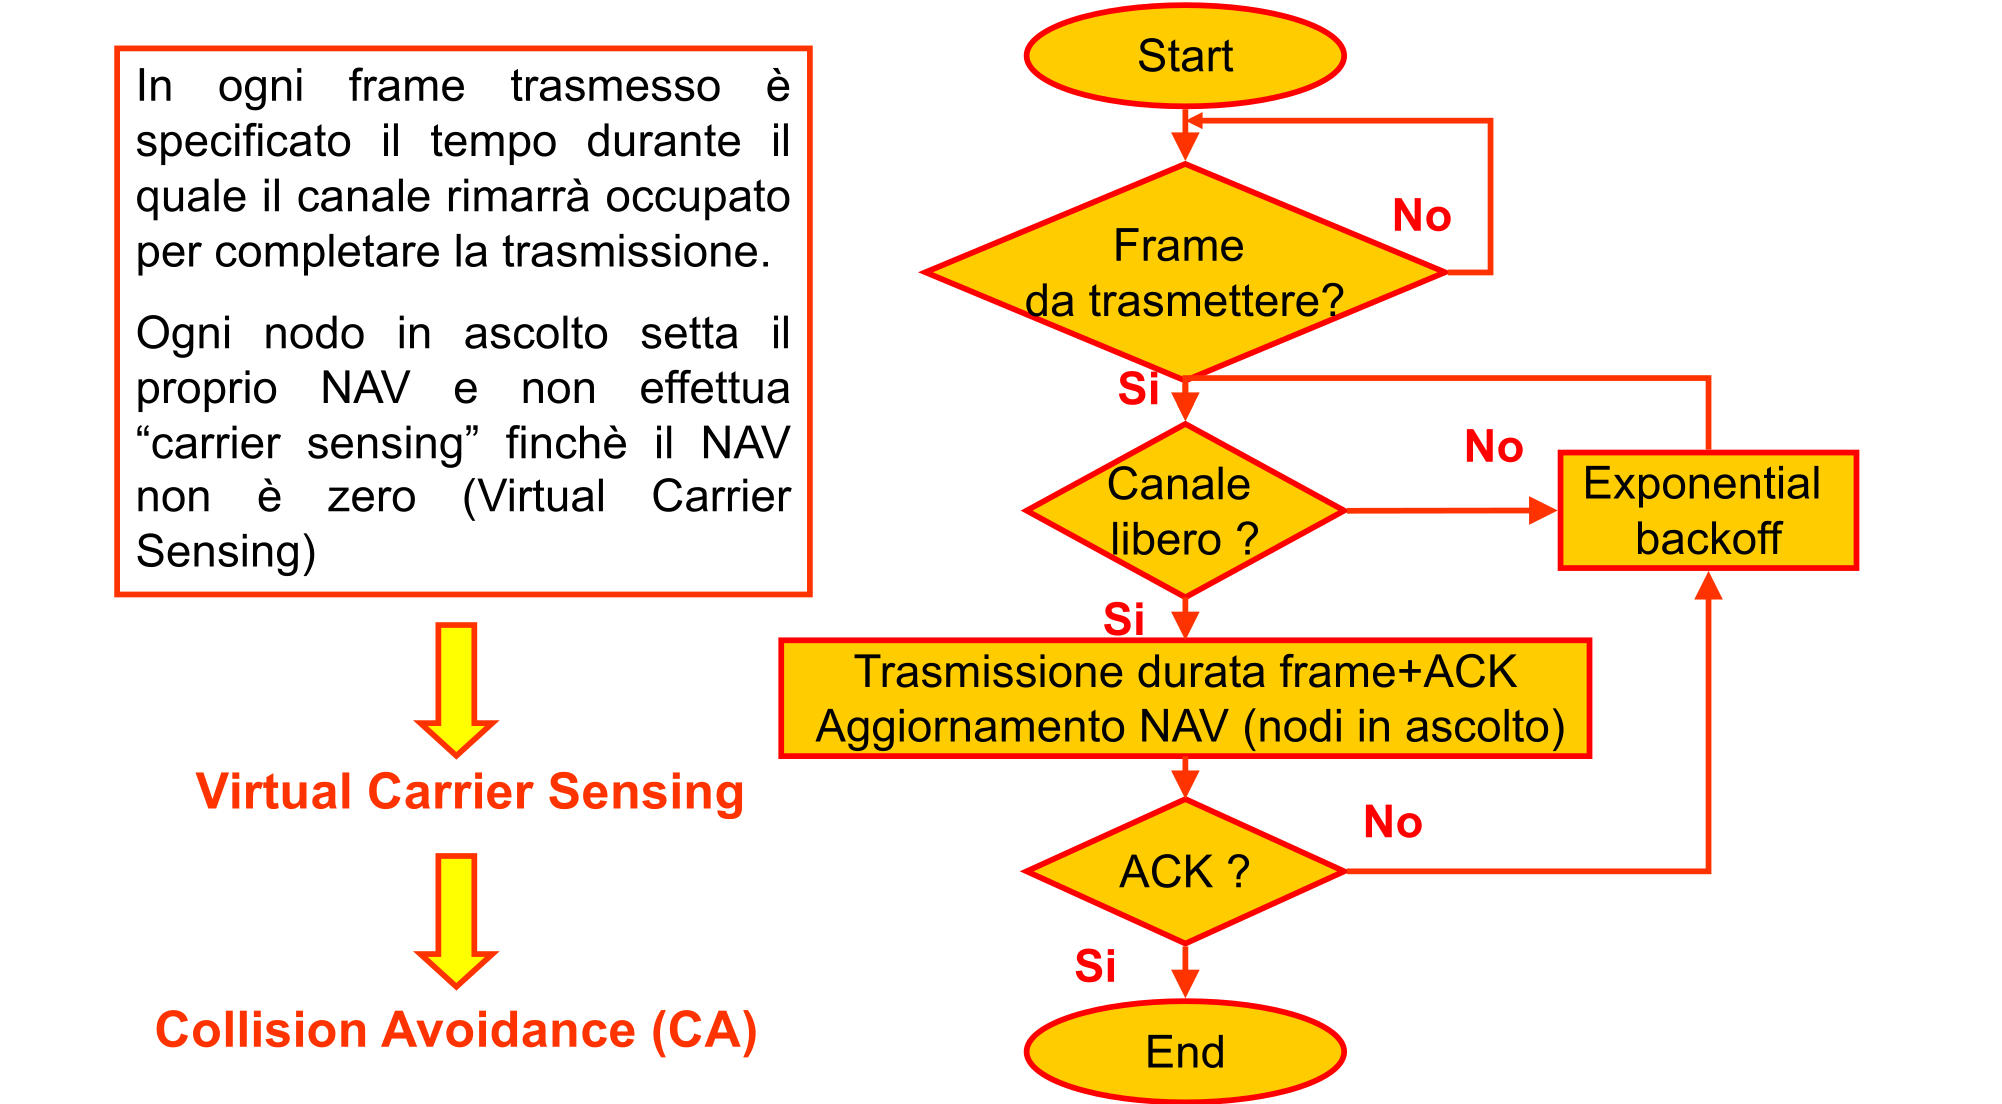
\includegraphics[width=0.65\textwidth]{images/csmaca.png}
    \caption{CSMA/CA}
    \label{fig:csma-ca}
\end{figure}